% Options for packages loaded elsewhere
\PassOptionsToPackage{unicode}{hyperref}
\PassOptionsToPackage{hyphens}{url}
%
\documentclass[
  ignorenonframetext,
]{beamer}
\usepackage{pgfpages}
\setbeamertemplate{caption}[numbered]
\setbeamertemplate{caption label separator}{: }
\setbeamercolor{caption name}{fg=normal text.fg}
\beamertemplatenavigationsymbolsempty
% Prevent slide breaks in the middle of a paragraph
\widowpenalties 1 10000
\raggedbottom
\setbeamertemplate{part page}{
  \centering
  \begin{beamercolorbox}[sep=16pt,center]{part title}
    \usebeamerfont{part title}\insertpart\par
  \end{beamercolorbox}
}
\setbeamertemplate{section page}{
  \centering
  \begin{beamercolorbox}[sep=12pt,center]{section title}
    \usebeamerfont{section title}\insertsection\par
  \end{beamercolorbox}
}
\setbeamertemplate{subsection page}{
  \centering
  \begin{beamercolorbox}[sep=8pt,center]{subsection title}
    \usebeamerfont{subsection title}\insertsubsection\par
  \end{beamercolorbox}
}
\AtBeginPart{
  \frame{\partpage}
}
\AtBeginSection{
  \ifbibliography
  \else
    \frame{\sectionpage}
  \fi
}
\AtBeginSubsection{
  \frame{\subsectionpage}
}

\usepackage{amsmath,amssymb}
\usepackage{iftex}
\ifPDFTeX
  \usepackage[T1]{fontenc}
  \usepackage[utf8]{inputenc}
  \usepackage{textcomp} % provide euro and other symbols
\else % if luatex or xetex
  \usepackage{unicode-math}
  \defaultfontfeatures{Scale=MatchLowercase}
  \defaultfontfeatures[\rmfamily]{Ligatures=TeX,Scale=1}
\fi
\usepackage{lmodern}
\usetheme[]{Berlin}
\ifPDFTeX\else  
    % xetex/luatex font selection
\fi
% Use upquote if available, for straight quotes in verbatim environments
\IfFileExists{upquote.sty}{\usepackage{upquote}}{}
\IfFileExists{microtype.sty}{% use microtype if available
  \usepackage[]{microtype}
  \UseMicrotypeSet[protrusion]{basicmath} % disable protrusion for tt fonts
}{}
\makeatletter
\@ifundefined{KOMAClassName}{% if non-KOMA class
  \IfFileExists{parskip.sty}{%
    \usepackage{parskip}
  }{% else
    \setlength{\parindent}{0pt}
    \setlength{\parskip}{6pt plus 2pt minus 1pt}}
}{% if KOMA class
  \KOMAoptions{parskip=half}}
\makeatother
\usepackage{xcolor}
\newif\ifbibliography
\setlength{\emergencystretch}{3em} % prevent overfull lines
\setcounter{secnumdepth}{-\maxdimen} % remove section numbering


\providecommand{\tightlist}{%
  \setlength{\itemsep}{0pt}\setlength{\parskip}{0pt}}\usepackage{longtable,booktabs,array}
\usepackage{calc} % for calculating minipage widths
\usepackage{caption}
% Make caption package work with longtable
\makeatletter
\def\fnum@table{\tablename~\thetable}
\makeatother
\usepackage{graphicx}
\makeatletter
\newsavebox\pandoc@box
\newcommand*\pandocbounded[1]{% scales image to fit in text height/width
  \sbox\pandoc@box{#1}%
  \Gscale@div\@tempa{\textheight}{\dimexpr\ht\pandoc@box+\dp\pandoc@box\relax}%
  \Gscale@div\@tempb{\linewidth}{\wd\pandoc@box}%
  \ifdim\@tempb\p@<\@tempa\p@\let\@tempa\@tempb\fi% select the smaller of both
  \ifdim\@tempa\p@<\p@\scalebox{\@tempa}{\usebox\pandoc@box}%
  \else\usebox{\pandoc@box}%
  \fi%
}
% Set default figure placement to htbp
\def\fps@figure{htbp}
\makeatother
% definitions for citeproc citations
\NewDocumentCommand\citeproctext{}{}
\NewDocumentCommand\citeproc{mm}{%
  \begingroup\def\citeproctext{#2}\cite{#1}\endgroup}
\makeatletter
 % allow citations to break across lines
 \let\@cite@ofmt\@firstofone
 % avoid brackets around text for \cite:
 \def\@biblabel#1{}
 \def\@cite#1#2{{#1\if@tempswa , #2\fi}}
\makeatother
\newlength{\cslhangindent}
\setlength{\cslhangindent}{1.5em}
\newlength{\csllabelwidth}
\setlength{\csllabelwidth}{3em}
\newenvironment{CSLReferences}[2] % #1 hanging-indent, #2 entry-spacing
 {\begin{list}{}{%
  \setlength{\itemindent}{0pt}
  \setlength{\leftmargin}{0pt}
  \setlength{\parsep}{0pt}
  % turn on hanging indent if param 1 is 1
  \ifodd #1
   \setlength{\leftmargin}{\cslhangindent}
   \setlength{\itemindent}{-1\cslhangindent}
  \fi
  % set entry spacing
  \setlength{\itemsep}{#2\baselineskip}}}
 {\end{list}}
\usepackage{calc}
\newcommand{\CSLBlock}[1]{\hfill\break\parbox[t]{\linewidth}{\strut\ignorespaces#1\strut}}
\newcommand{\CSLLeftMargin}[1]{\parbox[t]{\csllabelwidth}{\strut#1\strut}}
\newcommand{\CSLRightInline}[1]{\parbox[t]{\linewidth - \csllabelwidth}{\strut#1\strut}}
\newcommand{\CSLIndent}[1]{\hspace{\cslhangindent}#1}

\usepackage{amsmath}
\usepackage{mathtools}
\usepackage{tikz}
\usetikzlibrary{positioning}
\usetikzlibrary{decorations.pathreplacing}
\usepackage{algorithm}
\usepackage{algpseudocode}

\newcommand{\sgp}{\text{sgp}}
\newcommand{\rgp}{\text{rgp}}
\newcommand{\dgp}{\text{dgp}}
\renewcommand{\mod}{\text{mod}}

\setbeamertemplate{footline}{}
\makeatletter
\@ifpackageloaded{caption}{}{\usepackage{caption}}
\AtBeginDocument{%
\ifdefined\contentsname
  \renewcommand*\contentsname{Table of contents}
\else
  \newcommand\contentsname{Table of contents}
\fi
\ifdefined\listfigurename
  \renewcommand*\listfigurename{List of Figures}
\else
  \newcommand\listfigurename{List of Figures}
\fi
\ifdefined\listtablename
  \renewcommand*\listtablename{List of Tables}
\else
  \newcommand\listtablename{List of Tables}
\fi
\ifdefined\figurename
  \renewcommand*\figurename{Figure}
\else
  \newcommand\figurename{Figure}
\fi
\ifdefined\tablename
  \renewcommand*\tablename{Table}
\else
  \newcommand\tablename{Table}
\fi
}
\@ifpackageloaded{float}{}{\usepackage{float}}
\floatstyle{ruled}
\@ifundefined{c@chapter}{\newfloat{codelisting}{h}{lop}}{\newfloat{codelisting}{h}{lop}[chapter]}
\floatname{codelisting}{Listing}
\newcommand*\listoflistings{\listof{codelisting}{List of Listings}}
\makeatother
\makeatletter
\makeatother
\makeatletter
\@ifpackageloaded{caption}{}{\usepackage{caption}}
\@ifpackageloaded{subcaption}{}{\usepackage{subcaption}}
\makeatother

\usepackage{bookmark}

\IfFileExists{xurl.sty}{\usepackage{xurl}}{} % add URL line breaks if available
\urlstyle{same} % disable monospaced font for URLs
\hypersetup{
  pdftitle={Regimes' Characteristics and Time Series Forecasting},
  pdfauthor={Student: Ricardo Semião e Castro; Advisor: Prof.~Marcelo Fernandes},
  hidelinks,
  pdfcreator={LaTeX via pandoc}}


\title{Regimes' Characteristics and Time Series Forecasting}
\subtitle{FGV-EESP Masters' Thesis}
\author{Student: Ricardo Semião e Castro \and Advisor: Prof.~Marcelo
Fernandes}
\date{2025-10-09}

\begin{document}
\frame{\titlepage}


\section{Introduction}\label{introduction}

\begin{frame}{Motivation}
\phantomsection\label{motivation}
Interesting class of non-linear time series models -- regime switching
(RS) models:

\begin{itemize}
\tightlist
\item
  Allows for different behaviors (parameters) across different regimes.
\item
  Widely used in economics and finance, e.g., business cycles, market
  volatility.
\item
  Big diversity: Markov-switching, threshold models, smooth transition,
  etc.
\end{itemize}

It is important to understand the \emph{factors that influence their
performance}, and give \emph{practical recommendations} to
econometricians.
\end{frame}

\begin{frame}{Motivation}
\phantomsection\label{motivation-1}
\emph{Two focuses} in this work. \emph{The first} is more common in
forecasting econometrics:

\begin{itemize}
\tightlist
\item
  Exactly identifying the DGP is the exception, not the rule, we're
  looking for good approximators.
\item
  Thus, I analyze the sensitivity of each RS model to different
  mis-specifications.
\item
  Stylized results on how these models operate and interact with
  different DGPs.
\item
  Practical results on which models are more robust, which elements of
  the DGP are more important to identify.
\end{itemize}
\end{frame}

\begin{frame}{Motivation}
\phantomsection\label{motivation-2}
\emph{Two focuses} in this work. \emph{The second} is less orthodox and
specific to RS models:

\begin{itemize}
\tightlist
\item
  RS models estimate both the series and its regimes.
\item
  This allows for characterizing the regimes, and how different they are
  from each other.
\item
  This characterization might be informative for the model's
  performance.

  \begin{itemize}
  \tightlist
  \item
    E.g.: conditional average of the estimated regimes, for a DGP with
    different intercepts.
  \end{itemize}
\item
  Understand which characteristics are important in which contexts.
\end{itemize}
\end{frame}

\begin{frame}{General Methodology and Goals}
\phantomsection\label{general-methodology-and-goals}
\stepcounter{subsection}

The nature of this project is explorative.

I will simulate a diverse set of DGPs and try to find stylized facts
about:

\begin{itemize}
\tightlist
\item
  How each RS model adjusts to them.
\item
  How the characteristics of the estimated regimes relate to this
  adjustment.
\end{itemize}
\end{frame}

\begin{frame}{General Methodology and Goals}
\phantomsection\label{general-methodology-and-goals-1}
Common setup: establish a theoretical framework that describes all RS
models in a unified way.

\begin{itemize}
\tightlist
\item
  Separate the DGP into regime generating process (RGP) and series
  generating process (SGP).
\item
  Define a diverse menu of DGPs by varying these `ingredients'.

  \begin{itemize}
  \tightlist
  \item
    Cyclically updated based on the results of the exploratory analysis.
  \end{itemize}
\item
  Monte Carlo simulations to generate series, each applied to all
  considered models.
\end{itemize}

A partial goal is to create a very general and expandable theoretical
framework, simulation structure, and code implementation.
\end{frame}

\begin{frame}{General Methodology and Goals}
\phantomsection\label{general-methodology-and-goals-2}
For the first goal, I:

\begin{itemize}
\tightlist
\item
  Study the generated series

  \begin{itemize}
  \tightlist
  \item
    How each DGP `works' and how RGP and SGP interact.
  \end{itemize}
\item
  Study the estimation of the models.

  \begin{itemize}
  \tightlist
  \item
    Their fit, distribution of estimatives, and how these change across
    DGPs.
  \end{itemize}
\item
  Then, sistematize the correlations with regression analysis.

  \begin{itemize}
  \tightlist
  \item
    \(\text{RMSE} \sim \sgp \cdot \rgp \cdot \mod\).
  \end{itemize}
\end{itemize}
\end{frame}

\begin{frame}{General Methodology and Goals}
\phantomsection\label{general-methodology-and-goals-3}
For the second goal, I:

\begin{itemize}
\tightlist
\item
  Define the menu of regimes' characteristics that can be relevant in
  each DGP.

  \begin{itemize}
  \tightlist
  \item
    E.g. the conditional average for DGPs with intercept changes.
  \item
    Also cyclically updated.
  \end{itemize}
\item
  Calculate these metrics for the Monte Carlo results.
\item
  Study their behavior across DGPs and models.
\item
  Then, sistematize the correlations with regression analysis.

  \begin{itemize}
  \tightlist
  \item
    \(\text{RMSE} \sim \sgp \cdot \rgp \cdot \mod \cdot \text{metric}\).
  \end{itemize}
\end{itemize}
\end{frame}

\begin{frame}
\tableofcontents
\end{frame}

\begin{frame}
\textbf{Current stage of the work:}

\begin{itemize}
\tightlist
\item
  The theoretical framework and simulation structure was the focus, and
  is mostly finished.
\item
  The cycle of \emph{menu} \(\to\) \emph{exploratory analysis} \(\to\)
  \emph{systematic analysis} \(\to\) \emph{menu update} is ongoing.
\item
  The tools (graphs, tables, regressions) for the analysis have been
  created.

  \begin{itemize}
  \tightlist
  \item
    Some are presented here, for illustration.
  \item
    Most information hasn't been processed yet.
  \end{itemize}
\item
  Thus, the motivation and paths to follow are still abstract.
\end{itemize}
\end{frame}

\section{Theoretical Framework}\label{theoretical-framework}

\begin{frame}{Theoretical Framework}
\phantomsection\label{theoretical-framework-1}
Goal:

\begin{itemize}
\tightlist
\item
  Define the general structure of RS DGPs, in a unified mathematical
  representation.

  \begin{itemize}
  \tightlist
  \item
    An important idea is the separation of the DGP into RGP and SGP.
  \end{itemize}
\item
  Relate the concepts of models and metrics to it.
\item
  Describe the specific options considered in the menu.

  \begin{itemize}
  \tightlist
  \item
    And the motivations behind them.
  \item
    The hyperparametrization was not carefully chosen, yet.
  \end{itemize}
\end{itemize}
\end{frame}

\begin{frame}{Definitions - DGPs}
\phantomsection\label{definitions---dgps}
Let:

\begin{itemize}
\tightlist
\item
  \(y_t \in \mathbb{R}\) denote the series of interest

  \begin{itemize}
  \tightlist
  \item
    At time \(t \in 1:T\)\footnote<.->{Let
      \(a:b \coloneqq \{a, a+1, \dots, b\}\) for
      \(a \leq b \in \mathbb{Z}\), and
      \(y_{a:b} \coloneqq \{y_a, \dots, y_b\}\).}, \(T \in \mathbb{N}\).
  \end{itemize}
\item
  \(S \in \mathbb{N}\) denote the number of regimes.
\item
  The \emph{regime variable} is a vector of `weights' for each regime,
  indexed by \(r^s_t\), \(s \in 1:S\).
\end{itemize}
\end{frame}

\begin{frame}{Definitions - DGPs}
\phantomsection\label{definitions---dgps-1}
A DGP can be written in terms of a pair: \emph{regime generating
process} (RGP) and \emph{series generating process} (SGP). These are
functions with parameters \(\Theta_r\) and \(\Theta_y\), respectively,
such that:

\begin{equation}
\begin{array}{rrlllll}
    r_t &= \rgp(&y_{1:(t-1)}, &r_{t-1}, &t &;~ \Theta_r &)\\
    y_t &= \sgp(&y_{1:(t-1)}, &r_t,     &t &;~ \Theta_y &)\\
        &= \sgp(&y_{1:(t-1)}, &\rgp(y_{1:(t-1)}, r_{t-1}, t; \Theta_r), &t &;~ \Theta_y &)
\end{array}
\end{equation}

Notably, the number of regimes \(S\) is a parameter in \(\Theta_r\).
\end{frame}

\begin{frame}{Definitions - DGPs}
\phantomsection\label{definitions---dgps-2}
\(\Theta_y\) is actually a set of different parameters for each regime,
each indexed by \(\Theta^s_y\). This means that the SGP can be written
as:

\begin{equation}
    \sgp(y_{1:(t-1)}, r_t, t;~ \Theta_y) = \sum_{s = 1}^S f_{\sgp}(y_{1:(t-1)}, t;~ \Theta^s_y) \cdot r^s_t
\end{equation}

Each regime is weighted by the regime variable \(r^s_t\). In the
simplest case, this weight is binary (on vs.~off).

I refer to \(f_{\sgp}\) as the \emph{SGP functional
form}\footnote<.->{\(\Theta_y\) could encode different functional forms
  for each regime.}, or simply \emph{SGP}, and the set of parameters
\(\Theta_y\) as the \emph{regime nature}.
\end{frame}

\begin{frame}{Definitions - DGPs}
\phantomsection\label{definitions---dgps-3}
\begin{figure}[H]
    \centering
    \caption{The general RS DGP structure.}

    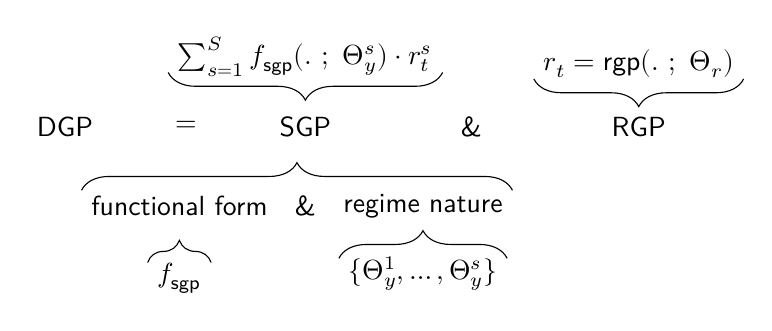
\begin{tikzpicture}[font=\sffamily]
    % Styles:
    \tikzset{mybrace/.style={decorate, decoration={brace, amplitude=10pt, raise=1.3ex}}}
    \tikzset{node distance = 0.25cm and 0.1cm}

    % Main nodes:
    \node[] (dgp) {DGP};
    \node[] (e)   [right = 0.8cm of dgp] {$=$};
    \node[] (sgp) [right = 0.8cm of e] {SGP};
    \node[] (p)   [right = 1.4cm of sgp] {\&};
    \node[] (rgp) [right = 1.4cm of p] {RGP};

    % Lower nodes:
    \node[] (p2)   [below = 0.5cm of sgp] {\&};
    \node[] (csgp) [left  = of p2] {functional form};
    \node[] (rsch) [right = of p2] {regime nature};

    % Math:
    \node[] (msgp)  [above = of sgp] {$\sum_{s = 1}^S f_{\sgp}(. ~;~ \Theta_y^s) \cdot r_t^s$};
    \node[] (mrgp)  [above = of rgp] {$r_t = \rgp(. ~;~ \Theta_r)$};
    \node[] (mcsgp) [below = 0.35cm of csgp] {$f_{\sgp}$};
    \node[] (mrsch) [below = of rsch] {$\{\Theta^1_y, \dots, \Theta^s_y\}$};

    % Braces using the defined style, add mirror in place:
    \draw[mybrace]         (csgp.west) -- (rsch.east);
    \draw[mybrace, decoration={mirror}] (mrgp.west) -- (mrgp.east);
    \draw[mybrace, decoration={mirror}] (msgp.west) -- (msgp.east);
    \draw[mybrace, decoration={amplitude=8pt}]         (mcsgp.west) -- (mcsgp.east);
    \draw[mybrace]         (mrsch.west) -- (mrsch.east);
    \end{tikzpicture}
\end{figure}

To construct a diverse set of DGPs, I combine different RGPs, SGPs, and
regime natures. Challenge: do so in a comprehensive yet systematic way.
\end{frame}

\begin{frame}{Definitions - DGPs}
\phantomsection\label{definitions---dgps-4}
I omitted the error term. For our purposes, consider the DGP as a
function that receives a vector of random erros\footnote<.->{This is a
  simplification, assuming the same error distribution across regimes.}:

\begin{equation}
    (y_{1:T},~ r_{1:T}) = \dgp(\varepsilon_{1:T};~ \Theta_r, \Theta_y)
\end{equation}

Let the menu of DGPs be \(P\) (for `processes').
\end{frame}

\begin{frame}{Definitions - Models}
\phantomsection\label{definitions---models}
Consider a model \(\mod\) as a function:

\begin{itemize}
\tightlist
\item
  With parameters \(\Theta_m\).
\item
  That generates the fitted values and \(h\)-step ahead predictions.
\item
  Of the series and regimes (and maybe some metadata).
\end{itemize}

\begin{equation}
    (\hat{y},~ \hat{r}) = \mod(y_{1:(T-h)} ~;~ \Theta_m)
\end{equation}

Notably, the number of estimated regimes \(\hat{S}\) is a parameter in
\(\Theta_m\), which differ from \(S\).

Let the set of models be \(M\) (for `models').
\end{frame}

\begin{frame}{Definitions - Metrics}
\phantomsection\label{definitions---metrics}
A conditional metric \(c\) is a function that:

\begin{itemize}
\tightlist
\item
  Receive a vector of series and a vector of regimes.
\item
  Are calculated separately for the set \(R_s\) of observations
  pertaining to each regime.

  \begin{itemize}
  \tightlist
  \item
    Non-stationarity imposes some limitations here.
  \item
    Continuous regime variables can be transformed into binary ones.
  \end{itemize}
\end{itemize}

\begin{equation}
\begin{array}{l}
    c: (y, r) \mapsto (R_s)_{s = 1}^S \mapsto \mathbb{R}^{S} \\
    R_s \coloneqq \left\{ y_t ~:~ r^s_t = \max\{r_t\} \right\}
\end{array}
\end{equation}

Let the set of metrics be \(C\) (for `criteria').
\end{frame}

\begin{frame}{Definitions - Metrics}
\phantomsection\label{definitions---metrics-1}
Metrics can be calculated in different ways:

\begin{itemize}
\tightlist
\item
  Metrics of the true values conditional on the true regimes:
  \(c(y, r)\).
\item
  Similarly for the estimated values: \(c(\hat{y}, \hat{r})\).
\item
  The difference between the two might be important.
\end{itemize}

The absolute value of a metric might be less important than its
dispersion across regimes.

\begin{itemize}
\tightlist
\item
  I.e., how different are the regimes in terms of that characteristic.
\end{itemize}

Some of this information are available to the econometrician, some are
not.
\end{frame}

\begin{frame}{Menu - SGP functional forms}
\phantomsection\label{menu---sgp-functional-forms}
\stepcounter{subsection}

The SGP is important in its interaction with the RGP, and is
context-specific (i.e.~GARCH models).

For now, a simple \(AR(1)\) is considered, for its wide use and ease of
estimation.

To simplify the metrics' analysis, I will focus on stationary models,
thus \(|\rho_1| < 1\).

\textbf{Stationary AR(1):}

\begin{equation}
\begin{array}{ll}
    &y_t(. ~;~ (\mu, \rho_1, \sigma)) = \mu + \rho_1 y_{t-1} + \sigma \cdot \varepsilon_t, ~~ \varepsilon_t \sim \mathcal{N}(0, 1)\\
    &|\rho_1| < 1, ~~ \sigma > 0
\end{array} \tag{SGP-AR(1)}
\end{equation}
\end{frame}

\begin{frame}{Menu - RGPs}
\phantomsection\label{menu---rgps}
To start, I will consider only two regimes, and some of the most common
RGPs: Structural Break, Self-Exciting Threshold, Smooth-Transition, and
Markov-Switching.

\textbf{Structural Break (SB):} Regime changes at specific time points
\(\tau \in (1:T)^{S-1}\).

\begin{equation}
\begin{array}{ll}
    &r^s_t(. ~;~ \tau) = \mathbb{1}(\tau'_{s-1} < t \leq \tau'_s), ~~ \forall s \in \{1, \dots S\}\\
    &\tau \in \mathbb{N}^{S-1}, ~~ \tau_{s} > \tau_{s-1} ~\forall s, ~~ \tau' = (0, \tau, T)\\
\end{array}\tag{RGP-SB}
\end{equation}

\textbf{Considered parametrizations:} ``Break at 1/2'' and ``Break at
2/3''.
\end{frame}

\begin{frame}{Menu - RGPs}
\phantomsection\label{menu---rgps-1}
\textbf{Self-Exciting Threshold (SET):} Regime changes when the
lagged/transformed\footnote<.->{For example, \(g(x) = |x|\) or
  \(g(x) = \Delta x\).} series \(g(y_{t-d})\) crosses some threshold
values \(\tau \in \mathbb{R}^{S-1}\).

\begin{equation}
\begin{array}{ll}
    &r^s_t(. ~;~ (\tau, d, g)) = \mathbb{1}(\tau'_{s-1} < g(y)_{t-d} \leq \tau'_s), ~~ \forall s \in \{1, \dots S\}\\
    &\tau \in \mathbb{R}^{S-1}, ~~ \tau_{s} > \tau_{s-1} ~\forall s, ~~ \tau' = (-\infty, \tau, \infty), ~~ d \in \mathbb{N}^*
\end{array}\tag{RGP-SET}
\end{equation}

\textbf{Considered parametrizations:} ``Threshold at 0'' and ``Threshold
at 0.5''.
\end{frame}

\begin{frame}{Menu - RGPs}
\phantomsection\label{menu---rgps-2}
\textbf{Smooth Transition (ST):} Regime changes smoothly, with a
CDF-like function \(g\) applied on the difference between the series and
the threshold \(\tau \in \mathbb{R}\). A generalization to \(S\) regimes
is equivalent to a neural network (Medeiros 2000). Parameters of \(g\)
can be estimated.

\begin{equation}
\begin{array}{ll}
    &r^1_t(. ~;~ (\tau, d, g)) = g(y_{t - d} - \tau),\\
    &r^2_t(. ~;~ (\tau, d, g)) = 1 - r^1_t(. ~;~ (\tau, d, g))\\
    &\tau \in \mathbb{R}, ~~ d \in \mathbb{N}^*
\end{array}\tag{RGP-ST}
\end{equation}

\textbf{Considered parametrizations:} ``LSTAR at 0'' and ``LSTAR at
0.5''.
\end{frame}

\begin{frame}{Menu - RGPs}
\phantomsection\label{menu---rgps-3}
\textbf{Markov-Switching (MS):} Regime changes stochastically, following
a Markov process with transition matrix
\(\Gamma \in [0, 1]^{S \times S}\).

\begin{equation}
\begin{array}{ll}
    &r^s_t(. ~;~ \Gamma) \sim P(r^s_t = 1 | r_{t-1}) \eqqcolon \Gamma_{s, r_{t-1}}\\
    &\Gamma \in [0, 1]^{S \times S}, ~~ \sum_{i=1}^S \Gamma_{s, i} = 1 ~\forall s\\
\end{array}\tag{RGP-MS}
\end{equation}

\textbf{Considered parametrizations:} ``Symmetric, High Persistence''
and ``Markov Symmetric, Low Persistence''.
\end{frame}

\begin{frame}{Menu - Models}
\phantomsection\label{menu---models}
All the RGPs above have model counterparts, and I will use all of them.
Additionally, more complex models such as random forest, neural
networks, or clustering-based models could be considered.

Common aspects of the hyperparameterization:

\begin{itemize}
\tightlist
\item
  The number of regimes is fixed, and varied across options.
\item
  All the coefficients are assumed to change across regimes.
\end{itemize}
\end{frame}

\begin{frame}{Menu - Models}
\phantomsection\label{menu---models-1}
\textbf{Structural Break AR:} Given \(\tau\), the model estimates
\(\mu\) and \(\rho_1\) via OLS in each regime. \(\tau\) is chosen by
minimizing the SSR over a grid search of breakpoints.

\textbf{Considered parametrizations:} No hyperparameterization needed.

\textbf{Seminal literature:} (Chow 1960), (Bai and Perron 1998).
\end{frame}

\begin{frame}{Menu - Models}
\phantomsection\label{menu---models-2}
\textbf{Self-Exciting Threshold AR:} Given \(\tau\) and \(d\), the model
estimates \(\mu\) and \(\rho_1\) via OLS in each regime. \(\tau\) and
\(d\) are chosen by minimizing the SSR over a grid search of breakpoints
and lags.

\textbf{Considered parametrizations:} The same transformation function
\(g\) as in the RGP will be considered. \(d\) will be fixed at 1.

\textbf{Seminal literature:} (Tong and Lim 1980).
\end{frame}

\begin{frame}{Menu - Models}
\phantomsection\label{menu---models-3}
\textbf{Smooth Transition AR:} Estimated via non-linear squares of the
residuals, over \(\mu\), \(\rho_1\) (for each regime), \(\tau\), and
\(\gamma\). Uses some numerical optimization.

\textbf{Considered parametrizations:} The same transformation function
\(g\) as in the RGP will be considered. Gamma will be fixed.

\textbf{Seminal literature:} (Teräsvirta 1994).
\end{frame}

\begin{frame}{Menu - Models}
\phantomsection\label{menu---models-4}
\textbf{Markov-Switching AR:} The MS-AR DGP is a state-space model,
which can then be related to filtering and smoothing techniques. The EM
algorithm uses Kalman to find smoothed probabilities of \(r\), which is
used to update the current guess of parameters via maximizing the
likelihood (given the probabilities). These two steps are iterated until
convergence.

\textbf{Considered parametrizations:} No hyperparameterization needed.

\textbf{Seminal literature:} (Hamilton 1989).
\end{frame}

\begin{frame}{Menu - Regime natures}
\phantomsection\label{menu---regime-natures}
The options are given below, in the format (\emph{parameter in regime
1}, \emph{parameter in regime 2}):

\begin{itemize}
\tightlist
\item
  \textbf{Mean (\(\mu\)) change:}

  \begin{itemize}
  \tightlist
  \item
    Small difference: (\(\mu = 0\), \(\mu = 0.5\))
  \item
    Large difference: (\(\mu = 0\), \(\mu = 2\))
  \end{itemize}
\item
  \textbf{Persistence (\(\rho_1\)) change:}

  \begin{itemize}
  \tightlist
  \item
    Small difference: (\(\rho_1 = 0.6\), \(\rho_1 = 0.4\))
  \item
    Large difference: (\(\rho_1 = 0.9\), \(\rho_1 = 0.1\))
  \end{itemize}
\item
  \textbf{Volatility (\(\sigma\)) change:}

  \begin{itemize}
  \tightlist
  \item
    Small difference: (\(\sigma = 1\), \(\sigma = 2\))
  \item
    Large difference: (\(\sigma = 1\), \(\sigma = 4\))
  \end{itemize}
\end{itemize}

Other options: sign switching, new lag introduction, etc.

Note that the regimes are always ordered increasingly by the parameter
of interest.
\end{frame}

\begin{frame}{Menu - Metrics}
\phantomsection\label{menu---metrics}
Each change specified by the regime natures is expected to affect the
series in a different way, and thus, be captured by different metrics.

First metric guess: the parameter of interest. In cases where more than
one parameter changes, this becomes less useful. I will consider other
metrics more `agnostic' over the DGP.

For the \emph{dispersion} of a metric, I consider the standard deviation
and average pairwise distance.
\end{frame}

\begin{frame}{Menu - Metrics}
\phantomsection\label{menu---metrics-1}
Mean (\(\mu\)) change:

\begin{itemize}
\tightlist
\item
  \(\widehat{\mu^s}\) and the \emph{conditional average}.
\item
  For the dispersion, direct measures of distance such as the
  \emph{silhouette score}.
\end{itemize}

Persistence (\(\rho_1\)) change:

\begin{itemize}
\tightlist
\item
  \(\widehat{\rho_1^s}\) and the \emph{conditional autocorrelation} of
  lag 1.
\end{itemize}

Volatility (\(\sigma\)) change:

\begin{itemize}
\tightlist
\item
  \(\widehat{\sigma^s}\).
\end{itemize}
\end{frame}

\begin{frame}{Menu - Metrics}
\phantomsection\label{menu---metrics-2}
Performance metrics:

\begin{itemize}
\tightlist
\item
  \(R^2\) for fit performance.
\item
  RMSE and MAPE for forecasting performance.
\end{itemize}

RGP metrics:

\begin{itemize}
\tightlist
\item
  Average duration of a regime.
\item
  Empirical transition matrix.
\item
  Midpoint between regimes.
\end{itemize}
\end{frame}

\section{Monte Carlo Simulations}\label{monte-carlo-simulations}

\begin{frame}{Simulation Structure}
\phantomsection\label{simulation-structure}
There are the following steps to perform the simulations:

\begin{enumerate}
\tightlist
\item
  Generate random errors for all the DGPs.
\item
  For each DGP and simulation, generate (\(y, r\)).
\item
  For each DGP, simulation, and model, obtain \((\hat{y},~ \hat{r})\).
\item
  For each DGP, simulation, and model, compute each metric.
\item
  Aggregate the metrics, performance information, and DGP and model
  descriptors into a dataset.
\end{enumerate}

This modular approach was chosen to fit in the exploratory nature of the
work.

The implementation is done in R, and is available in
\href{https://github.com/ricardo-semiao/article-regime-id-performance}{github.com/ricardo-semiao/article-regime-id-performance}.
The code is modular, reproducible, and expandable.
\end{frame}

\begin{frame}{Simulation Structure}
\phantomsection\label{simulation-structure-1}
For the forecast performance, I focus on \(1\)-step ahead predictions.
Local projections could be considered.

To increase the number of forecast points per simulation, i predict
\(10\) \(1\)-step ahead predictions,
\(\hat{y}_{T-h} \mid y_{1:(T - h - 1)}\).

The current parameters of the simulation are as follows:

\begin{itemize}
\tightlist
\item
  Number of simulations: \(I = 500\).
\item
  Total number of observations: \(T = 120\).
\item
  Burn-in period: \(10\).
\item
  Forecast horizon: \(10\) predictions of \(1\)-step ahead values.
\end{itemize}

Let \(i \in 1:I\), \(I \in \mathbb{N}\) be the simulation index.
\end{frame}

\begin{frame}{Simulating Errors}
\phantomsection\label{simulating-errors}
The set of DGPs \(P\) is the cartesian product of the considered RGPs,
SGPs, and regime natures.

I create \(|P| \cdot I\) sets of random error vectors, each of size
\(1:T\). They are generated in parallel, using
\href{https://www.numbercrunch.de/trng/}{TRNG}. Let \(\Epsilon\) denote
the set of all errors.

Let \(\Epsilon_{p, i}\) denote the vector of errors generated for the
\(p\)-th DGP and the \(i\)-th simulation.

Error diagnostics are presented in the appendix.
\end{frame}

\begin{frame}{Simulating Series}
\phantomsection\label{simulating-series}
Let \(Y\) and \(R\) denote the sets of generated series and regime
variables for each \(p\) and \(i\). They are computed given
\(\Epsilon_{p, i}\):

\begin{algorithm}[H]
\begin{algorithmic}[1]
    \State Initialize $Y$ and $R$
    \For{$(p, i)$ \textbf{in} $(1:|P|) \times (1:I)$}
        \State Spawn a new parallel task
        \State $Y_{p, i},~ R_{p, i} \gets P_p(\Epsilon_{p, i})$
\EndFor
\end{algorithmic}
\end{algorithm}

The nesting order here and in the next sections were chosen to optimize
the parallelization.
\end{frame}

\begin{frame}{Estimating Models}
\phantomsection\label{estimating-models}
For each simulation, I estimate each model, generating the sets
\(\hat{Y}\) and \(\hat{R}\). The models are trained using only
\(y_{(10 + 1):(T-10)}\). They are computed given \(Y_{p, i}\) and
\(R_{p, i}\):

\begin{algorithm}[H]
\begin{algorithmic}[1]
    \State Initialize $\hat{Y}$ and $\hat{R}$
    \For{$(p, i)$ \textbf{in} $(1:|P|) \times (1:I)$}
        \State Spawn a new parallel task
        \For{$m$ \textbf{in} $1:|M|$}
            \State $\hat{Y}_{p, i, m},~ \hat{R}_{p, i, m} \gets M_m(Y_{p, i})$
        \EndFor
    \EndFor
\end{algorithmic}
\end{algorithm}
\end{frame}

\begin{frame}{Estimating Metrics}
\phantomsection\label{estimating-metrics}
Then, for each model, the metrics and other meta-information are
calculated and stored as columns of a dataset \(D\). Each line of \(D\)
is an observation \((p, i, m)\), each column a metric \((c)\).

\begin{algorithm}[H]
\begin{algorithmic}[1]
    \State Initialize $D$
    \For{$(p, i, m)$ \textbf{in} $(1:|P|) \times (1:I) \times (1:|M|)$}
        \State Spawn a new parallel task
        \For{$c$ \textbf{in} $1:|C|$}
            \State $D_{(p, i, m),~ c} \gets C_c(\hat{Y}_{p, i, m})$
        \EndFor
        \State $D \gets$ performance metrics and DGP/model categorical descriptors
    \EndFor
\end{algorithmic}
\end{algorithm}
\end{frame}

\begin{frame}{Simulation Dimensions}
\phantomsection\label{simulation-dimensions}
\begin{itemize}
\tightlist
\item
  There are \(48\) DGPs considered.

  \begin{itemize}
  \tightlist
  \item
    \(1\) SGP, \(6\) regime natures, and \(8\) options of RGP.
  \end{itemize}
\item
  Each is simulated \(500\) times, yielding \(24,000\) series.
\item
  For each simulation, \(4\) models are estimated, yielding \(96,000\).

  \begin{itemize}
  \tightlist
  \item
    \(946\) had convergence problems and were removed, leaving
    \(95,054\) estimated models.
  \item
    The total of estimated time points is \(11,407,680\).
  \item
    The biggest bottleneck, but with this numbers takes about 2 hours to
    run.
  \end{itemize}
\item
  There are \(17\) metrics, \(2\) regimes, and \(3,231,836\) metrics
  calculated.

  \begin{itemize}
  \tightlist
  \item
    \(2\) performance metrics. Also \(3\) SGP metrics, \(0\) RGP
    metrics, and \(2\) parameters.
  \item
    Calculated with the true, estimated values, and their difference.
  \end{itemize}
\item
  \(4,154\) -- the current number of lines of R code in the repository.
\end{itemize}
\end{frame}

\section{Exploratory Analysis}\label{exploratory-analysis}

\begin{frame}
Recalling the \textbf{current stage of the work:}

\begin{itemize}
\tightlist
\item
  The tools (graphs, tables, regressions) for the analysis have been
  created.

  \begin{itemize}
  \tightlist
  \item
    Some are presented here, for illustration.
  \item
    Most information hasn't been processed yet.
  \end{itemize}
\item
  My goal today is to present these tools and the type of analysis I
  intend to do.
\end{itemize}
\end{frame}

\begin{frame}{Exploratory Analysis}
\phantomsection\label{exploratory-analysis-1}
Goals:

\begin{itemize}
\tightlist
\item
  Explore the data.
\item
  Learn how each DGP behaves, and how the models interact with them.
\item
  Motivate the modeling decisions for the systematic analysis.
\end{itemize}

Obs: the regimes are ordered increasingly by the parameter that changes.
This is only possible in the single-parameter change regime natures.
\end{frame}

\begin{frame}{Series - Values}
\phantomsection\label{series---values}
Figure~\ref{fig-sim-v1} show the series' values and distribution, for
the MS-AR(1) model, with a symmetric high-persistence transition matrix.

Each row represents a different regime nature, with only \(\mu\)
changing, only \(\rho_1\) changing, and only \(\sigma\) changing,
respectively. The grey area is the burn-in period.

We can see how:

\begin{itemize}
\tightlist
\item
  The high persistence of regimes is indeed present.
\item
  The change in intercept and volatility are clear.
\item
  The higher \(\rho_1\) conditions a more volatile regime
\end{itemize}
\end{frame}

\begin{frame}{Series - Values}
\phantomsection\label{series---values-1}
\begin{figure}

\caption{\label{fig-sim-v1}Values and distribution of MS-AR(1) DGP}

\centering{

\pandocbounded{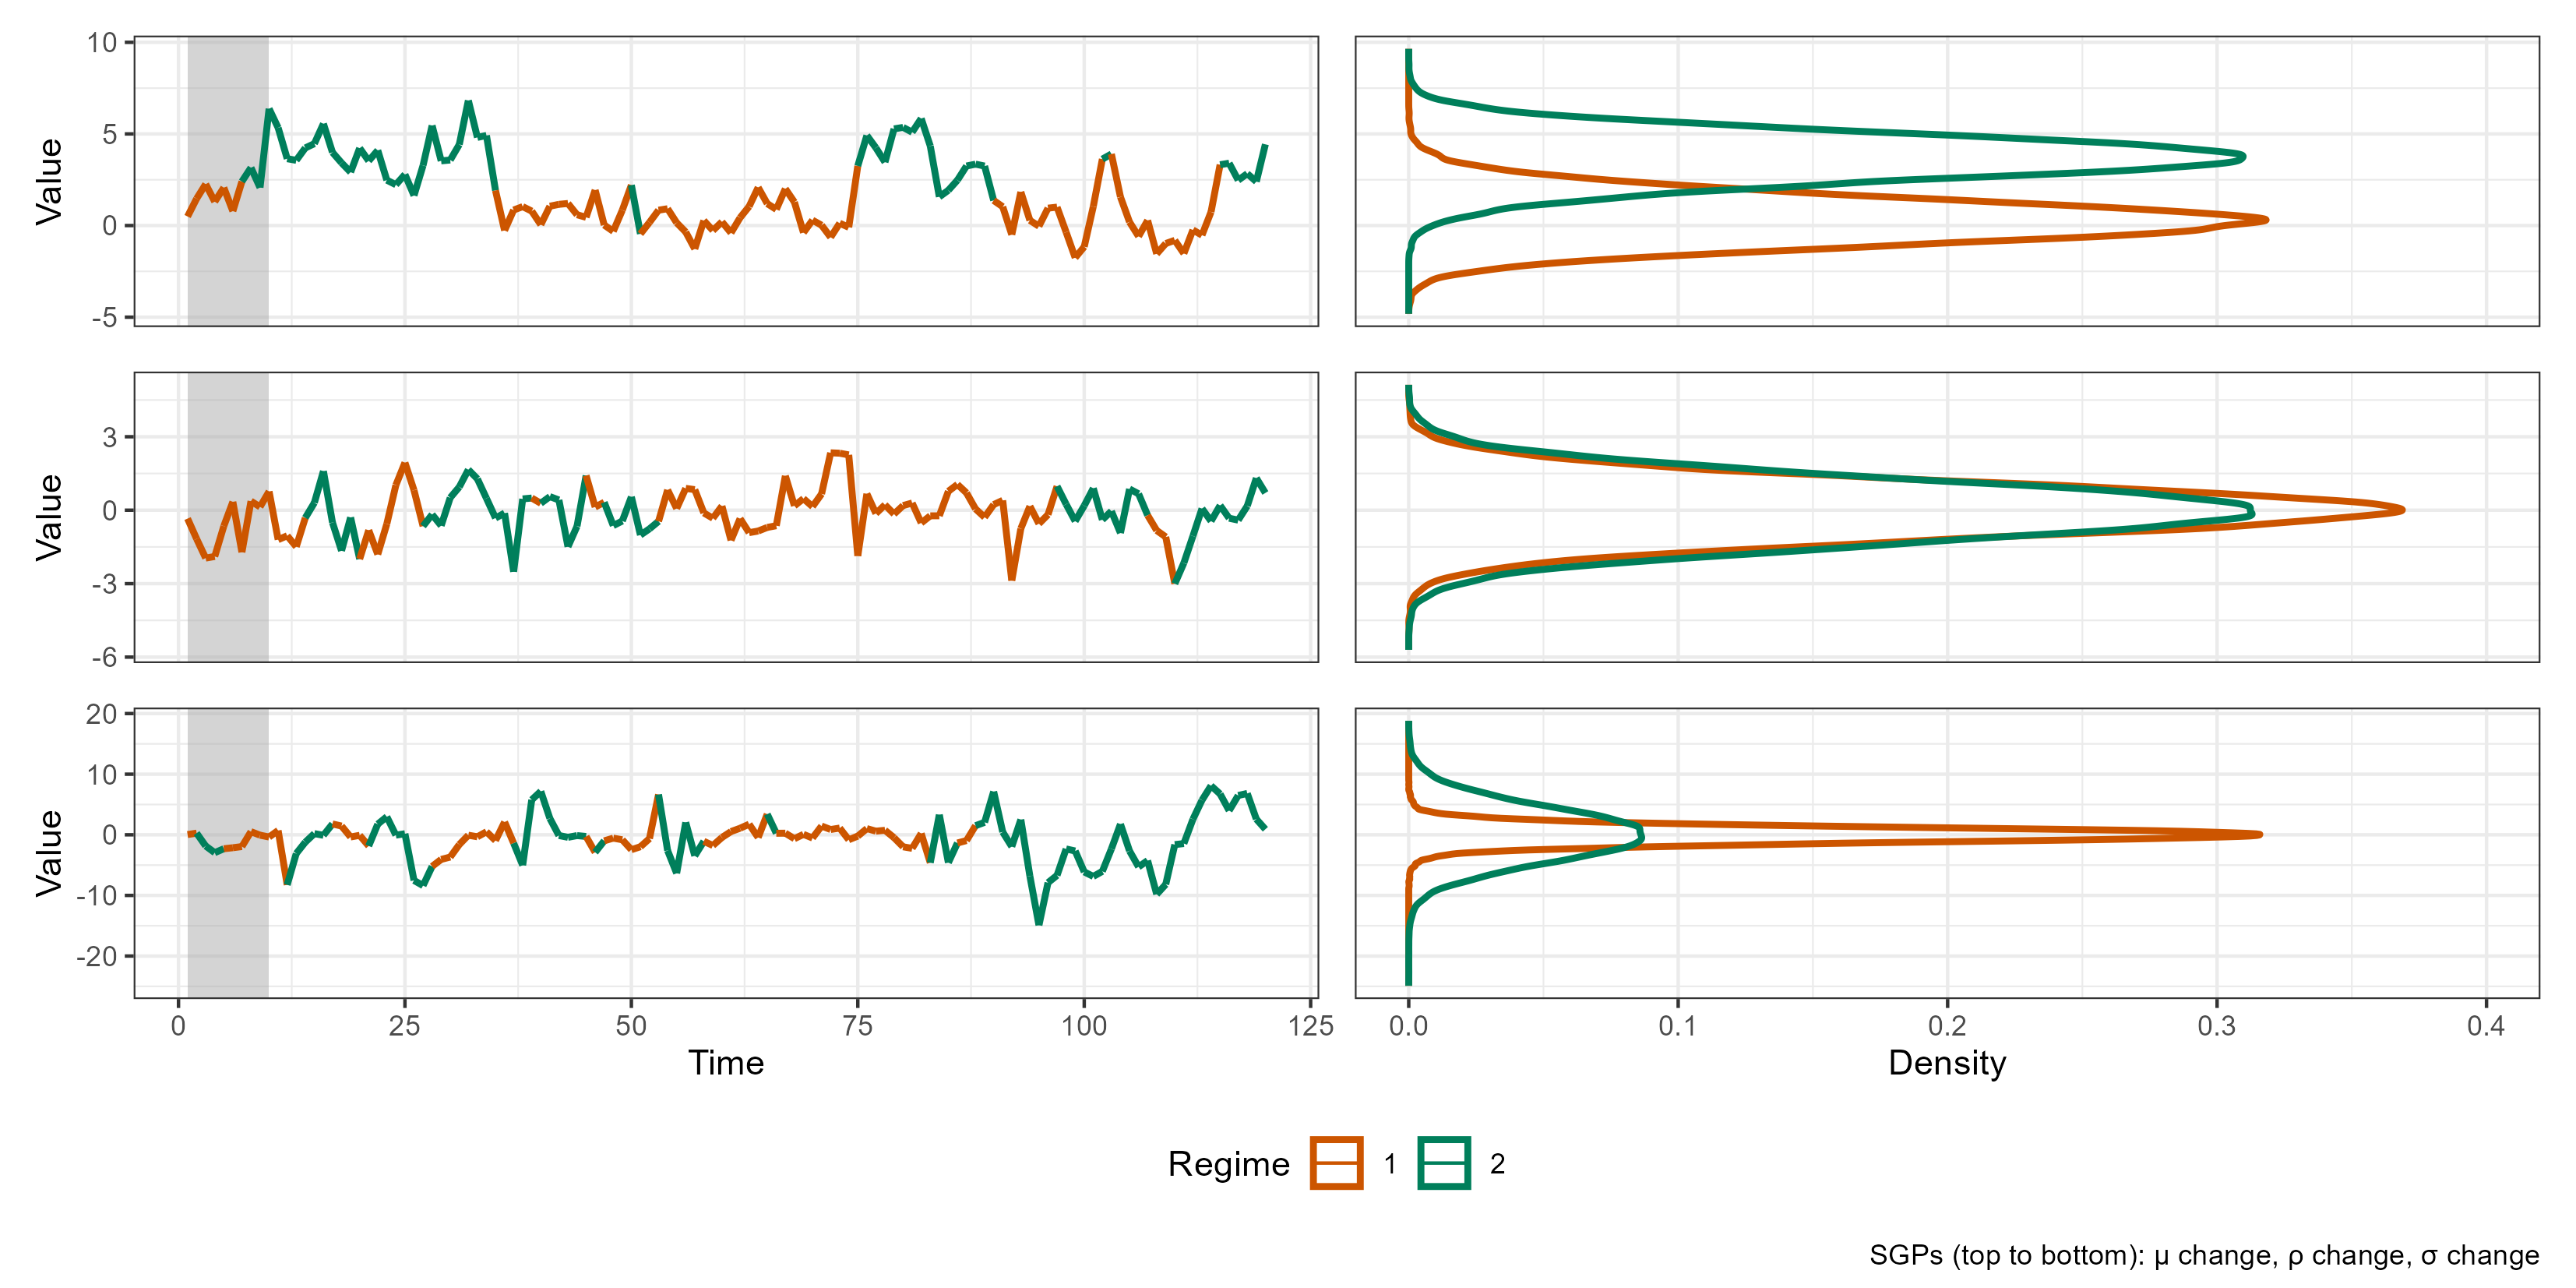
\includegraphics[keepaspectratio]{../../outputs/simulations/values-r2_markov_symm_high.png}}

}

\end{figure}%
\end{frame}

\begin{frame}{Series - Values}
\phantomsection\label{series---values-2}
Figure~\ref{fig-sim-v2} shows the series for the SET-AR(1) model, with a
threshold at 0.

The interaction between RGP and the regime nature is evident:

\begin{itemize}
\tightlist
\item
  The higher \(\mu\) makes the series likely to stay in regime 2.
\item
  The higher volatility and \(\rho_1\) when above \(0\) conditions a
  higher level for the series in the second regime.
\end{itemize}

Many other observations could be made.
\end{frame}

\begin{frame}{Series - Values}
\phantomsection\label{series---values-3}
\begin{figure}

\caption{\label{fig-sim-v2}Values of SET-AR(1) model}

\centering{

\pandocbounded{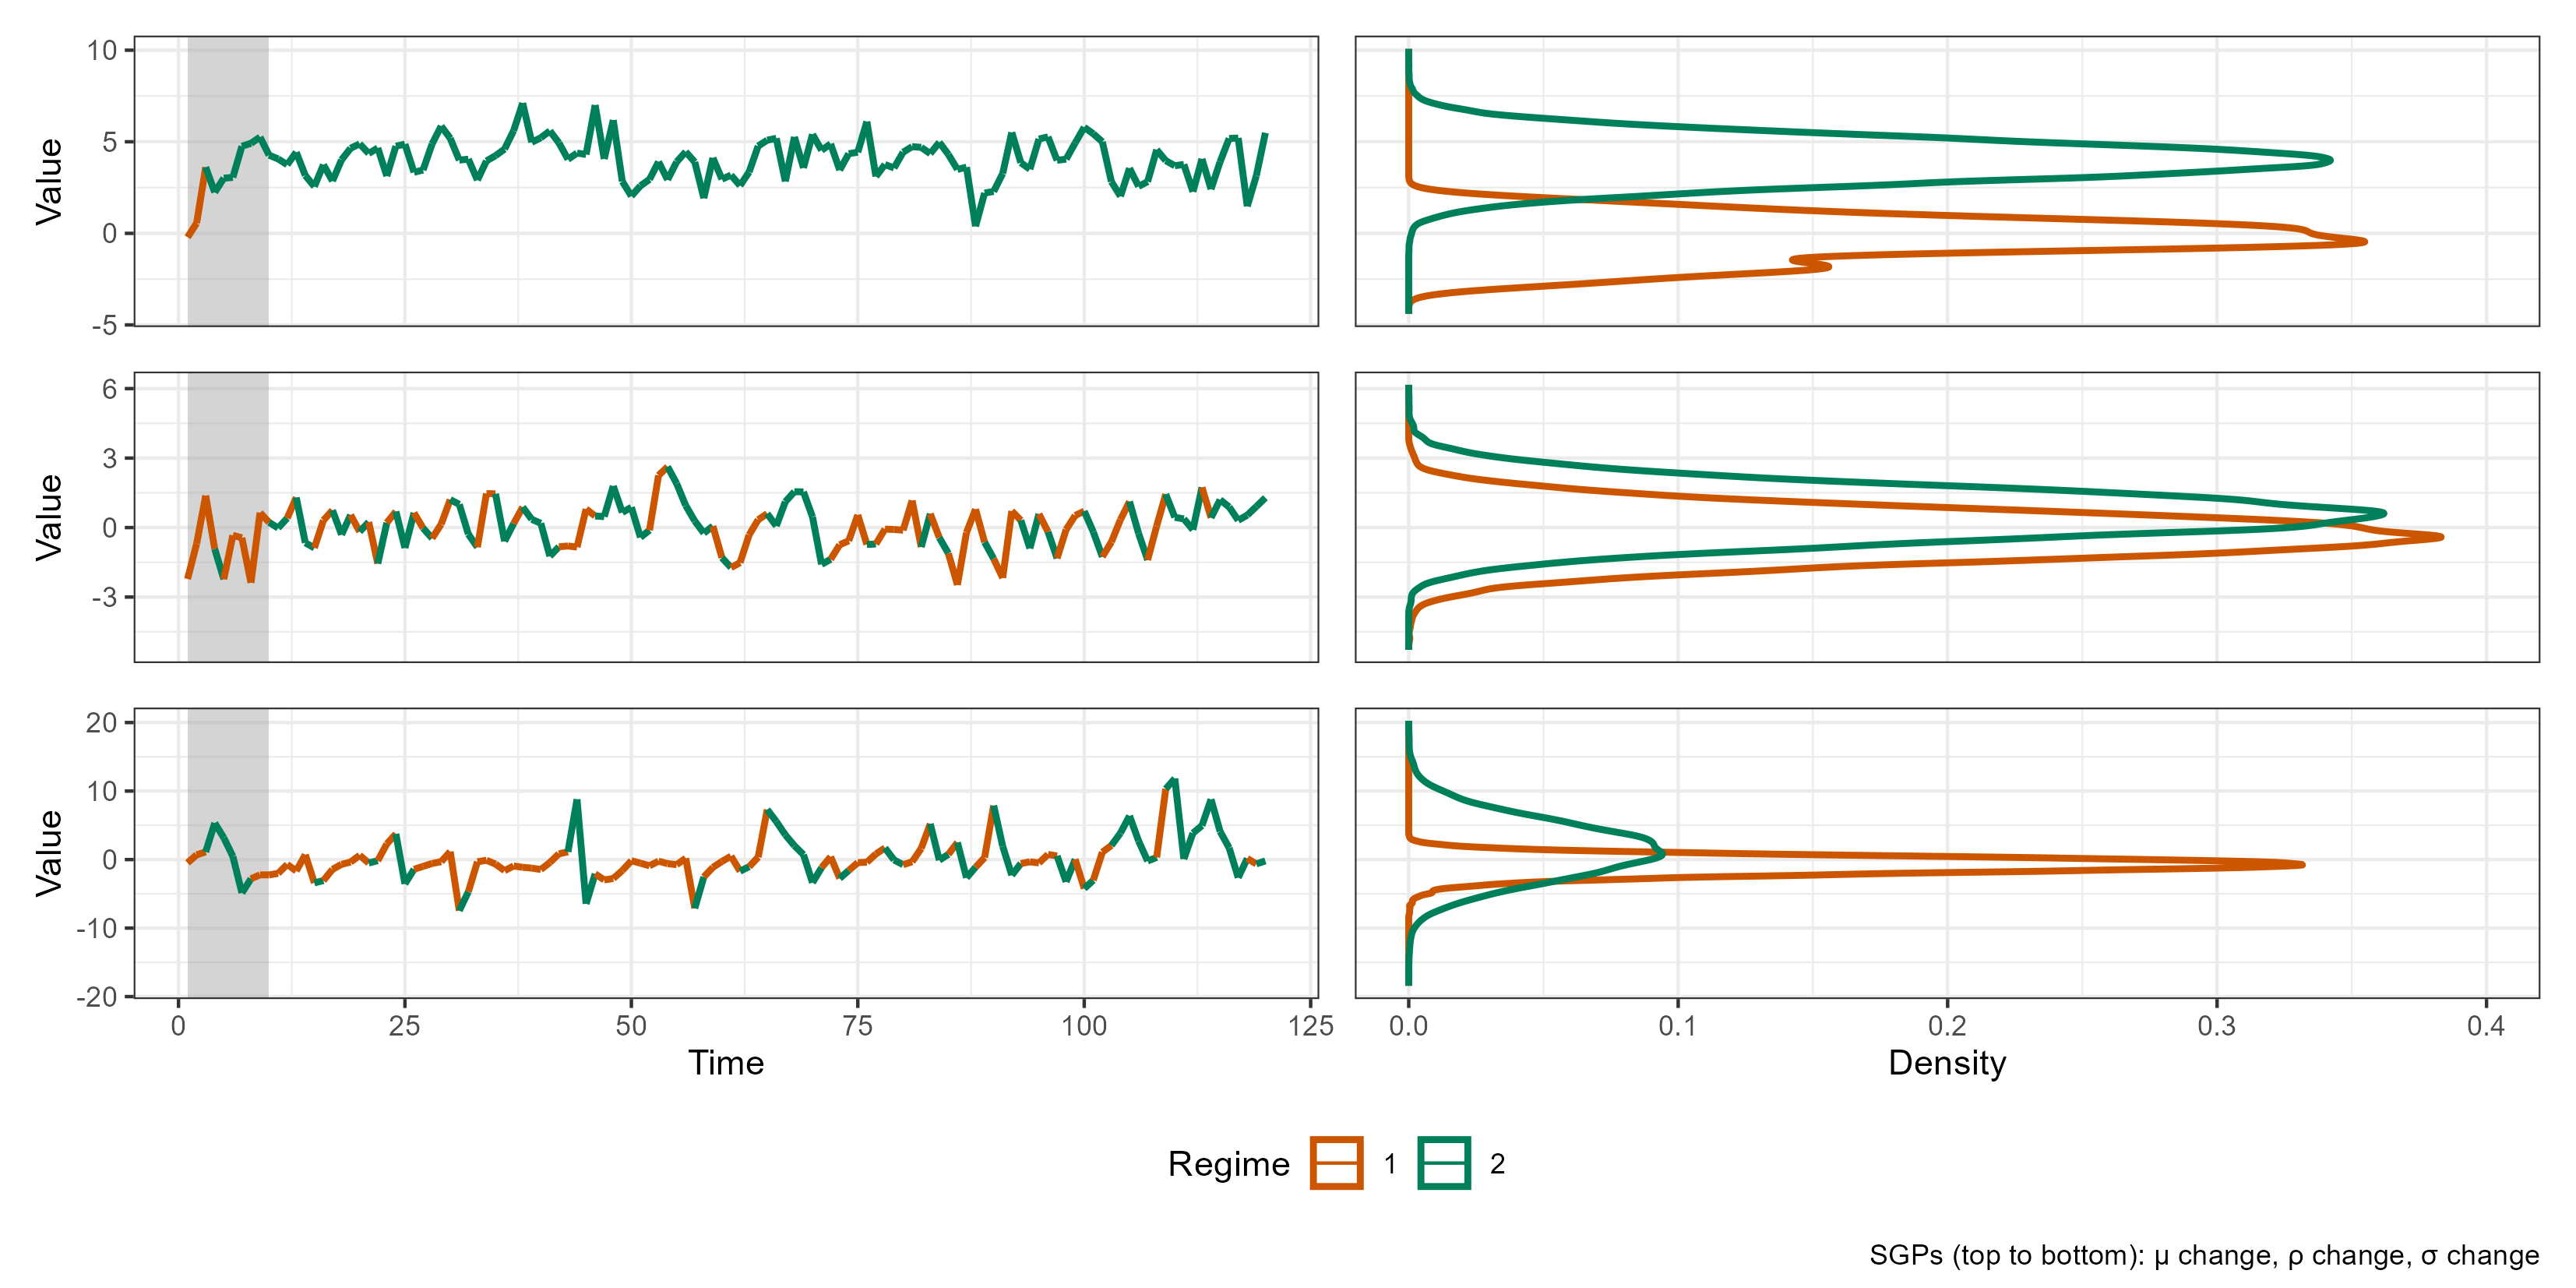
\includegraphics[keepaspectratio]{../../outputs/simulations/values-r2_threshold_x_0.png}}

}

\end{figure}%
\end{frame}

\begin{frame}{Series - Metrics}
\phantomsection\label{series---metrics}
Here, I check:

\begin{itemize}
\tightlist
\item
  How the metrics behave in the simulated series.

  \begin{itemize}
  \tightlist
  \item
    Useful to rethink which metrics are relevant for each regime nature.
  \end{itemize}
\item
  How the metrics converge across \(T\).

  \begin{itemize}
  \tightlist
  \item
    If our chosen \(T\) were too small, even metrics that well
    characterize the regimes would not do so.
  \item
    To analyze convergence, I plot the metrics calculated up to time
    \(t\), for all \(t \in 1:T\).
  \item
    Lines for multiple simulations can be combined to analyze
    convergence across \(I\).
  \end{itemize}
\end{itemize}
\end{frame}

\begin{frame}{Series - Metrics}
\phantomsection\label{series---metrics-1}
Figure~\ref{fig-sim-m1} shows the metrics for the SET-AR(1) model, with
a threshold at 0.

Each row represents a different regime nature, thus a different
conditional metric (mean, ACF(1), and SD, respectively).

In general, the metrics seem to converge and to characterize the
regimes.
\end{frame}

\begin{frame}{Series - Metrics}
\phantomsection\label{series---metrics-2}
\begin{figure}

\caption{\label{fig-sim-m1}SGP metrics of SET-AR(1) model}

\centering{

\pandocbounded{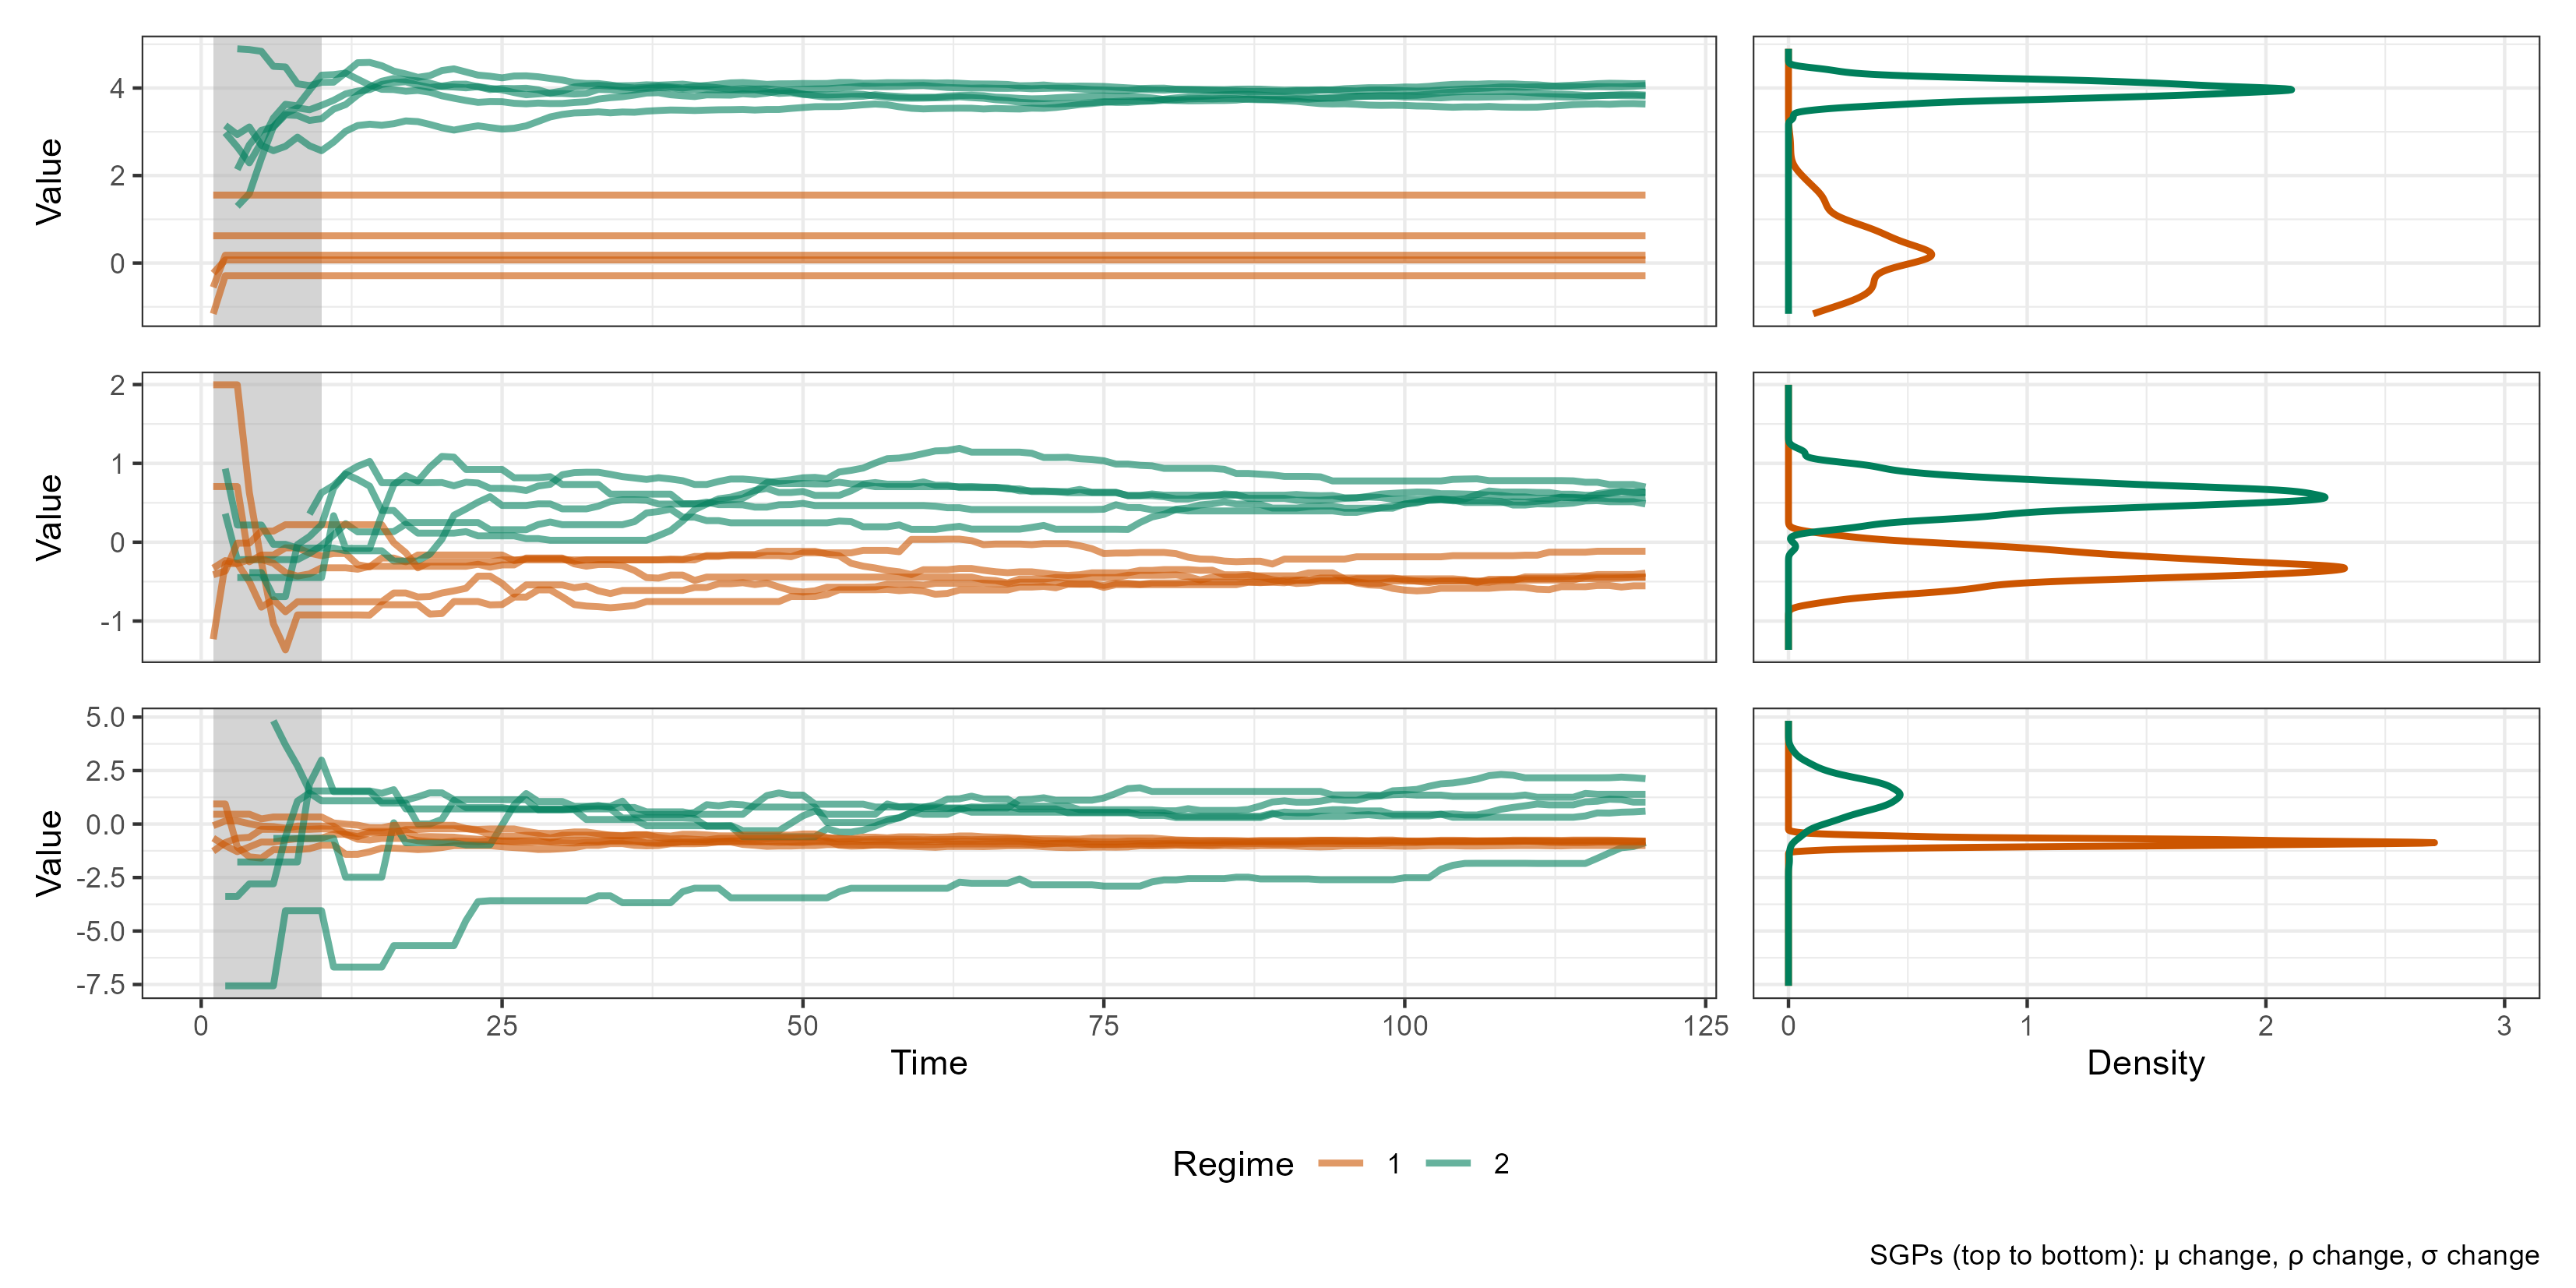
\includegraphics[keepaspectratio]{../../outputs/simulations/stats_sgp-r2_threshold_x_0.png}}

}

\end{figure}%
\end{frame}

\begin{frame}{Series - Metrics}
\phantomsection\label{series---metrics-3}
Figure~\ref{fig-sim-m2} shows a metric for the RGP itself, for the
MS-AR(1). Specifically, the empirical (non-)transition probability for
each regime.

We can see how the metrics converge to the true value (\(0.8\)), across
all regime natures.
\end{frame}

\begin{frame}{Series - Metrics}
\phantomsection\label{series---metrics-4}
\begin{figure}

\caption{\label{fig-sim-m2}RGP metrics of MS-AR(1) model}

\centering{

\pandocbounded{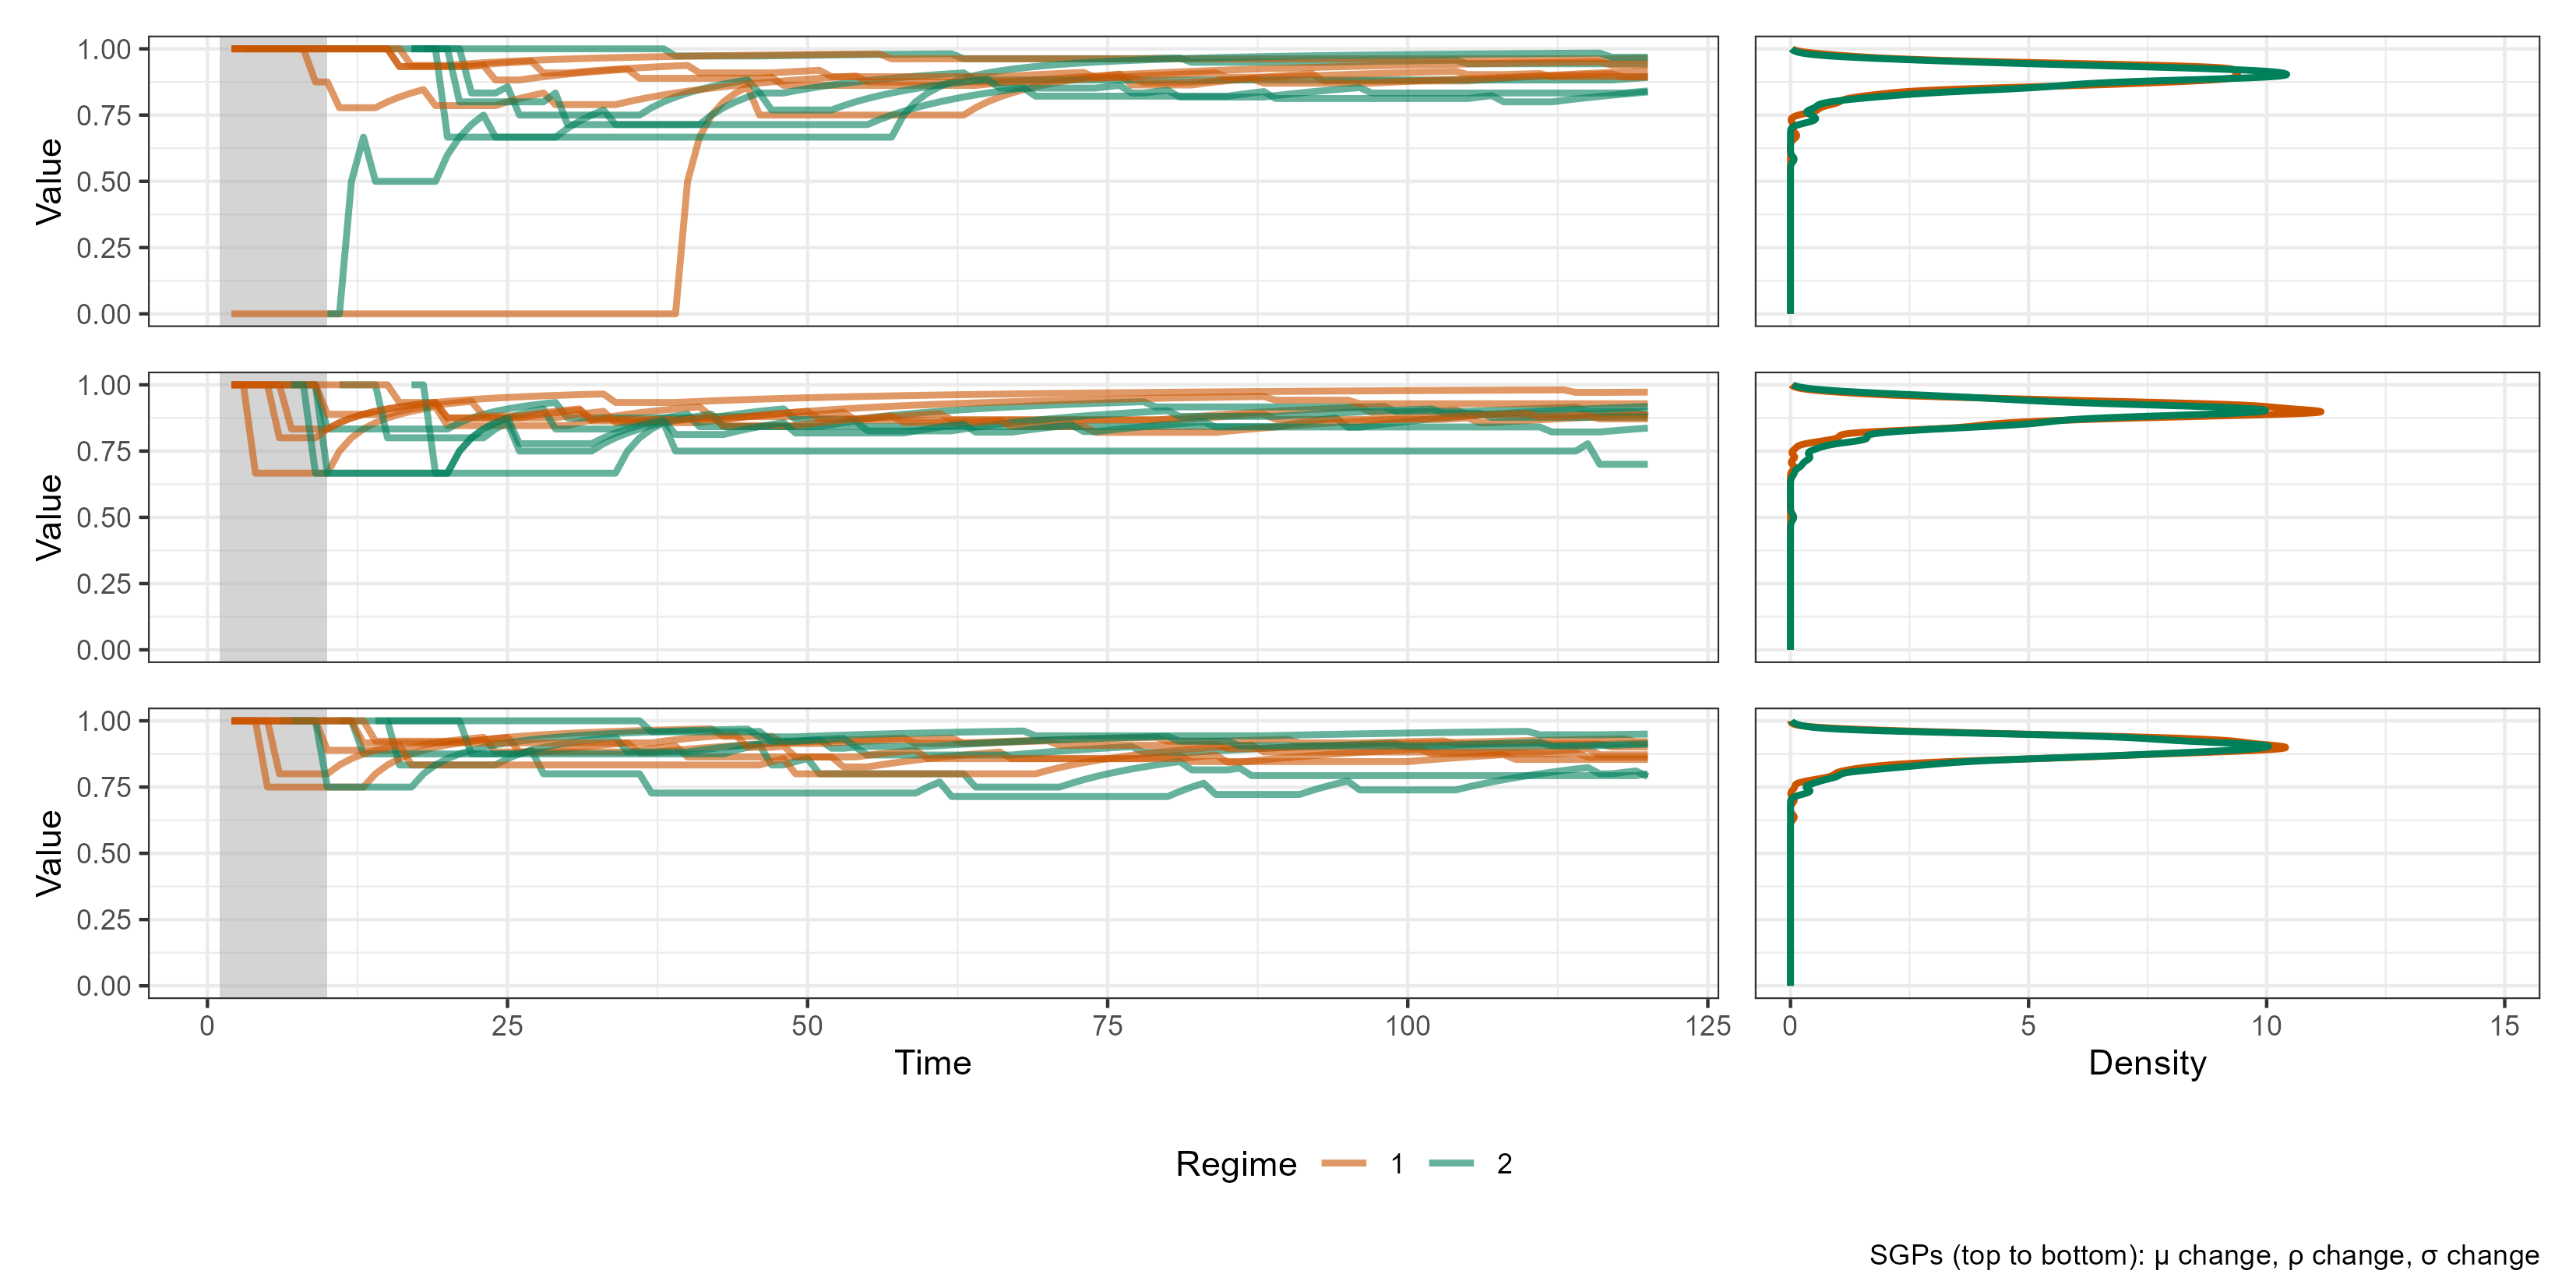
\includegraphics[keepaspectratio]{../../outputs/simulations/stats_rpg-r2_markov_symm_high.png}}

}

\end{figure}%
\end{frame}

\begin{frame}{Series - Metrics}
\phantomsection\label{series---metrics-5}
In a more systematic way, I:

\begin{itemize}
\tightlist
\item
  Tabulate the average and standard deviation of the metrics, across
  DGPs.
\item
  Test the null hypothesis that the metrics do not vary across regimes
  (ANOVA).

  \begin{itemize}
  \tightlist
  \item
    Note that the power of this test is directly related to the number
    \(I\) of simulations.
  \end{itemize}
\end{itemize}
\end{frame}

\begin{frame}{Series - Metrics}
\phantomsection\label{series---metrics-6}
\begin{table}[t]
\fontsize{12.0pt}{14.0pt}\selectfont
\begin{tabular*}{\linewidth}{@{\extracolsep{\fill}}ccrrrrl}
\toprule
 &  & \multicolumn{2}{c}{R1} & \multicolumn{2}{c}{R2} & ANOVA \\ 
\cmidrule(lr){3-4} \cmidrule(lr){5-6} \cmidrule(lr){7-7}
SGP & RGP & Mean & SD & Mean & SD & P-value \\ 
\midrule\addlinespace[2.5pt]
\ensuremath{\mu} (big change) & Markov (symm., high persist.) & 0.30 & 0.27 & 3.60 & 0.29 & 0.0e+00*** \\ 
\ensuremath{\mu} (big change) & S-break (at 1/2) & -0.01 & 0.28 & 3.92 & 0.24 & 0.0e+00*** \\ 
\ensuremath{\mu} (big change) & Threshold (x, at 0) & 0.17 & 0.79 & 3.96 & 0.19 & 0.0e+00*** \\ 
\ensuremath{\mu} (big change) & LSTAR (at 0) & 1.14 & 0.11 & 0.98 & 0.23 & 6.2e-43*** \\ 
\ensuremath{\rho} (big change) & Markov (symm., high persist.) & 0.32 & 0.13 & 0.48 & 0.14 & 2.9e-70*** \\ 
\ensuremath{\rho} (big change) & S-break (at 1/2) & 0.36 & 0.13 & 0.55 & 0.11 & 1.0e-105*** \\ 
\ensuremath{\rho} (big change) & Threshold (x, at 0) & 0.13 & 0.14 & 0.26 & 0.13 & 4.7e-49*** \\ 
\ensuremath{\rho} (big change) & LSTAR (at 0) & 0.15 & 0.14 & 0.24 & 0.14 & 1.5e-27*** \\ 
\ensuremath{\sigma} (big change) & Markov (symm., high persist.) & 1.35 & 0.21 & 4.40 & 0.55 & 0.0e+00*** \\ 
\ensuremath{\sigma} (big change) & S-break (at 1/2) & 1.13 & 0.13 & 4.50 & 0.48 & 0.0e+00*** \\ 
\ensuremath{\sigma} (big change) & Threshold (x, at 0) & 1.27 & 0.13 & 4.16 & 0.49 & 0.0e+00*** \\ 
\ensuremath{\sigma} (big change) & LSTAR (at 0) & 1.77 & 0.16 & 3.66 & 0.47 & 0.0e+00*** \\ 
\bottomrule
\end{tabular*}
\end{table}

\end{frame}

\begin{frame}{Models}
\phantomsection\label{models}
\stepcounter{subsection}

Now, similar analisis can be done, which enables us to understand how
the models interact with the DGPs.

\begin{itemize}
\tightlist
\item
  Instead of comparing the true and estimated series' values, I plot the
  residuals.

  \begin{itemize}
  \tightlist
  \item
    Besides separating them by regimes, I also separate them by
    \(\mathbb{1}(\hat{r}_t = r_t)\).
  \end{itemize}
\item
  The same metrics can be calculated for the estimated counterparts.

  \begin{itemize}
  \tightlist
  \item
    I analyze if the models capture the regimes' characteristics, across
    mis-specifications.
  \end{itemize}
\item
  Additionally, check the coefficients' distributions vs.~true values.

  \begin{itemize}
  \tightlist
  \item
    Useful to note how coefficients that \emph{shouldn't} change
    compensate mis-specifications.
  \end{itemize}
\end{itemize}
\end{frame}

\begin{frame}{Models - Values}
\phantomsection\label{models---values}
Figure~\ref{fig-mod-v1} shows the residuals and their distribution for
the MS-AR(1) model, estimated on top of an SB RGP.
Figure~\ref{fig-mod-v2} color the regimes by `correctness'.

It appears that the estimated regime relates more to the residual level
than its actual correctness.

The differences in average and volatility are expected, and no
difference can be seen in the autocorrelation change.

Again, in a more systematic way, I tabulate the average and standard
deviation of the residuals across estimated regimes.
\end{frame}

\begin{frame}{Models - Values}
\phantomsection\label{models---values-1}
\begin{figure}

\caption{\label{fig-mod-v1}Residuals of MS-AR(1) estimating a SB-AR(1)}

\centering{

\pandocbounded{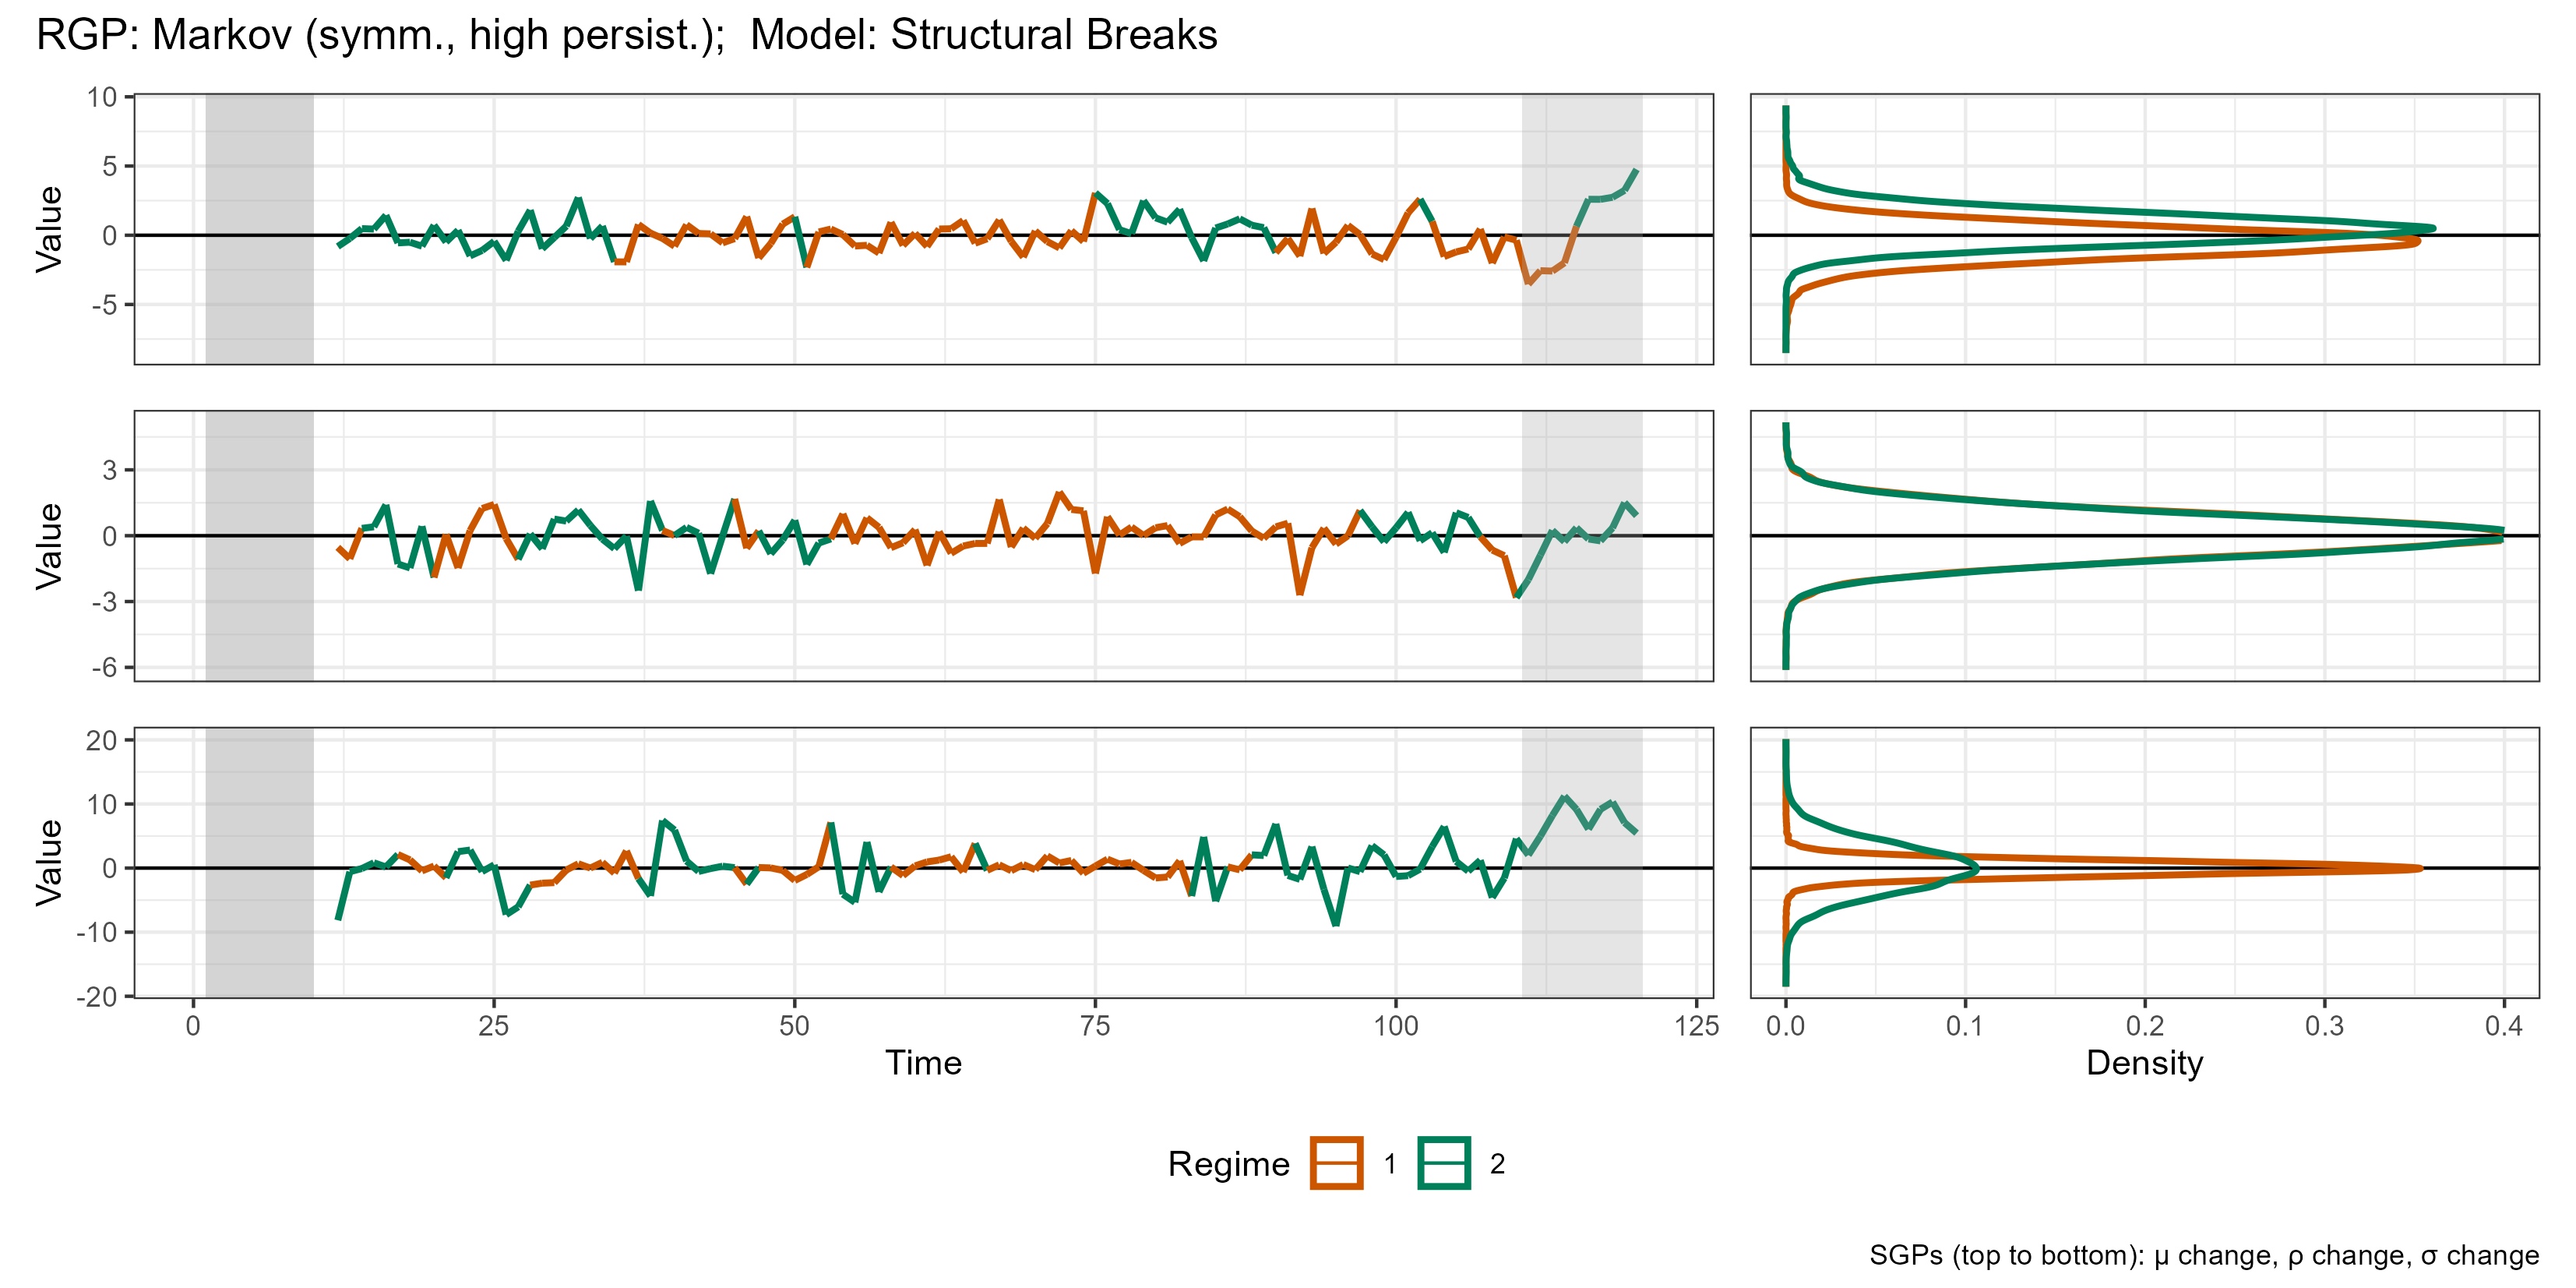
\includegraphics[keepaspectratio]{../../outputs/estimations/residuals-r2_markov_symm_high-r2_sbreak-a.png}}

}

\end{figure}%
\end{frame}

\begin{frame}{Models - Values}
\phantomsection\label{models---values-2}
\begin{figure}

\caption{\label{fig-mod-v2}Residuals of MS-AR(1) estimating a SB-AR(1)}

\centering{

\pandocbounded{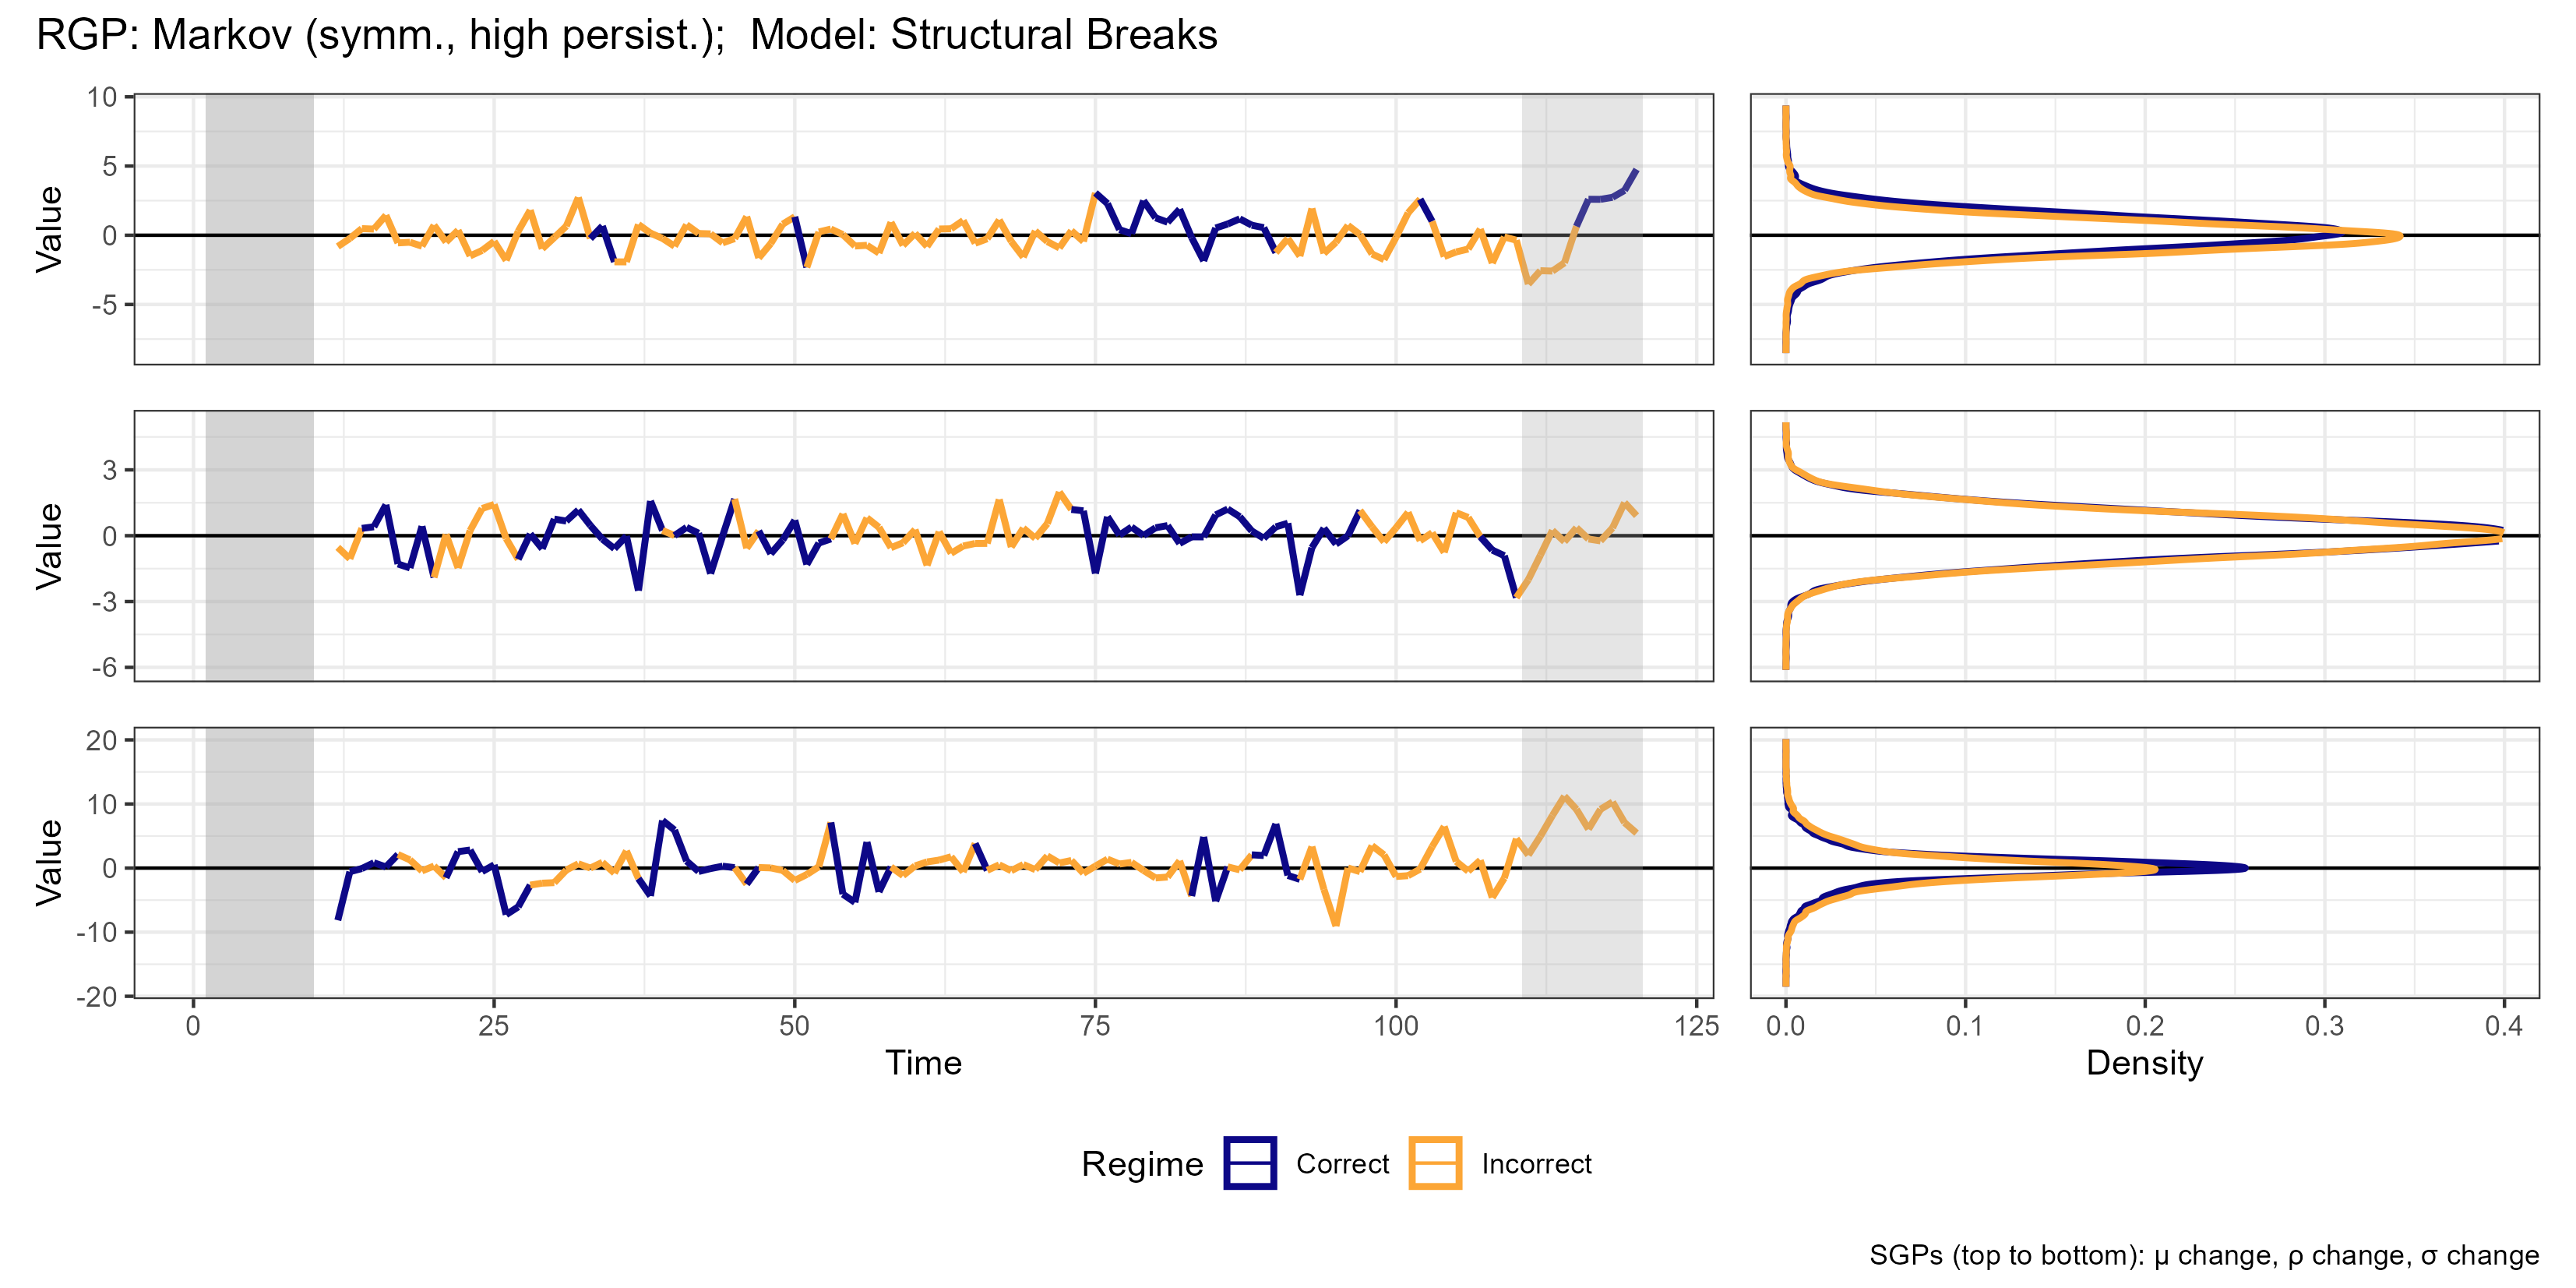
\includegraphics[keepaspectratio]{../../outputs/estimations/residuals-r2_markov_symm_high-r2_sbreak-na.png}}

}

\end{figure}%
\end{frame}

\begin{frame}{Models - Values}
\phantomsection\label{models---values-3}
\begin{table}[t]
\fontsize{8pt}{8pt}\selectfont
\begin{tabular*}{\linewidth}{@{\extracolsep{\fill}}ccrrrrl}
\toprule
 &  & \multicolumn{2}{c}{R1} & \multicolumn{2}{c}{R2} & ANOVA \\ 
\cmidrule(lr){3-4} \cmidrule(lr){5-6} \cmidrule(lr){7-7}
SGP & RGP & Mean & SD & Mean & SD & P-value \\ 
\midrule\addlinespace[2.5pt]
\ensuremath{\mu}   & Markov (symm., high persist.) & 0.65 & 18.32 & 0.11 & 0.21 & 5.0e-01 \\ 
\ensuremath{\mu}   & S-break (at 1/2) & -0.14 & 0.09 & 0.03 & 0.10 & 3.2e-127*** \\ 
\ensuremath{\mu}   & Threshold (x, at 0) & -0.07 & 0.15 & -0.03 & 0.14 & 4.1e-05*** \\ 
\ensuremath{\mu}   & LSTAR (at 0) & -0.11 & 0.11 & 0.08 & 0.13 & 5.1e-110*** \\ 
\ensuremath{\rho}  & Markov (symm., high persist.) & -0.01 & 0.14 & -0.00 & 0.16 & 6.4e-01 \\ 
\ensuremath{\rho}  & S-break (at 1/2) & -0.01 & 0.14 & -0.01 & 0.39 & 5.9e-01 \\ 
\ensuremath{\rho}  & Threshold (x, at 0) & 0.18 & 4.32 & 1.26 & 28.20 & 4.0e-01 \\ 
\ensuremath{\rho}  & LSTAR (at 0) & -0.01 & 0.14 & 0.02 & 0.15 & 7.1e-03*** \\ 
\ensuremath{\sigma} & Markov (symm., high persist.) & -0.07 & 0.28 & -0.09 & 3.01 & 8.7e-01 \\ 
%\ensuremath{\sigma} & S-break (at 1/2) & 1539.50 & 34417.52 & 0.24 & 2.62 & 3.2e-01 \\ 
\ensuremath{\sigma} & Threshold (x, at 0) & -0.37 & 0.19 & 0.37 & 0.17 & 0.0e+00*** \\ 
\ensuremath{\sigma} & LSTAR (at 0) & 0.32 & 0.13 & -0.37 & 0.23 & 0.0e+00*** \\ 
\bottomrule
\end{tabular*}
\end{table}

\end{frame}

\begin{frame}{Models - Coefficients}
\phantomsection\label{models---coefficients}
Here, I analyze if the models capture the coefficients and their
difference across regimes.

Note that this might not be a necessary condition for a good
approximation.

Figure~\ref{fig-mod-c1} follows the same model from before and shows:

\begin{itemize}
\tightlist
\item
  The distribution of each estimated coefficient (\(\mu\) and
  \(\rho_1\))
\item
  While the dotted lines give the true values.
\end{itemize}
\end{frame}

\begin{frame}{Models - Coefficients}
\phantomsection\label{models---coefficients-1}
\begin{figure}

\caption{\label{fig-mod-c1}Coefficients of MS-AR(1) estimating a
SB-AR(1)}

\centering{

\pandocbounded{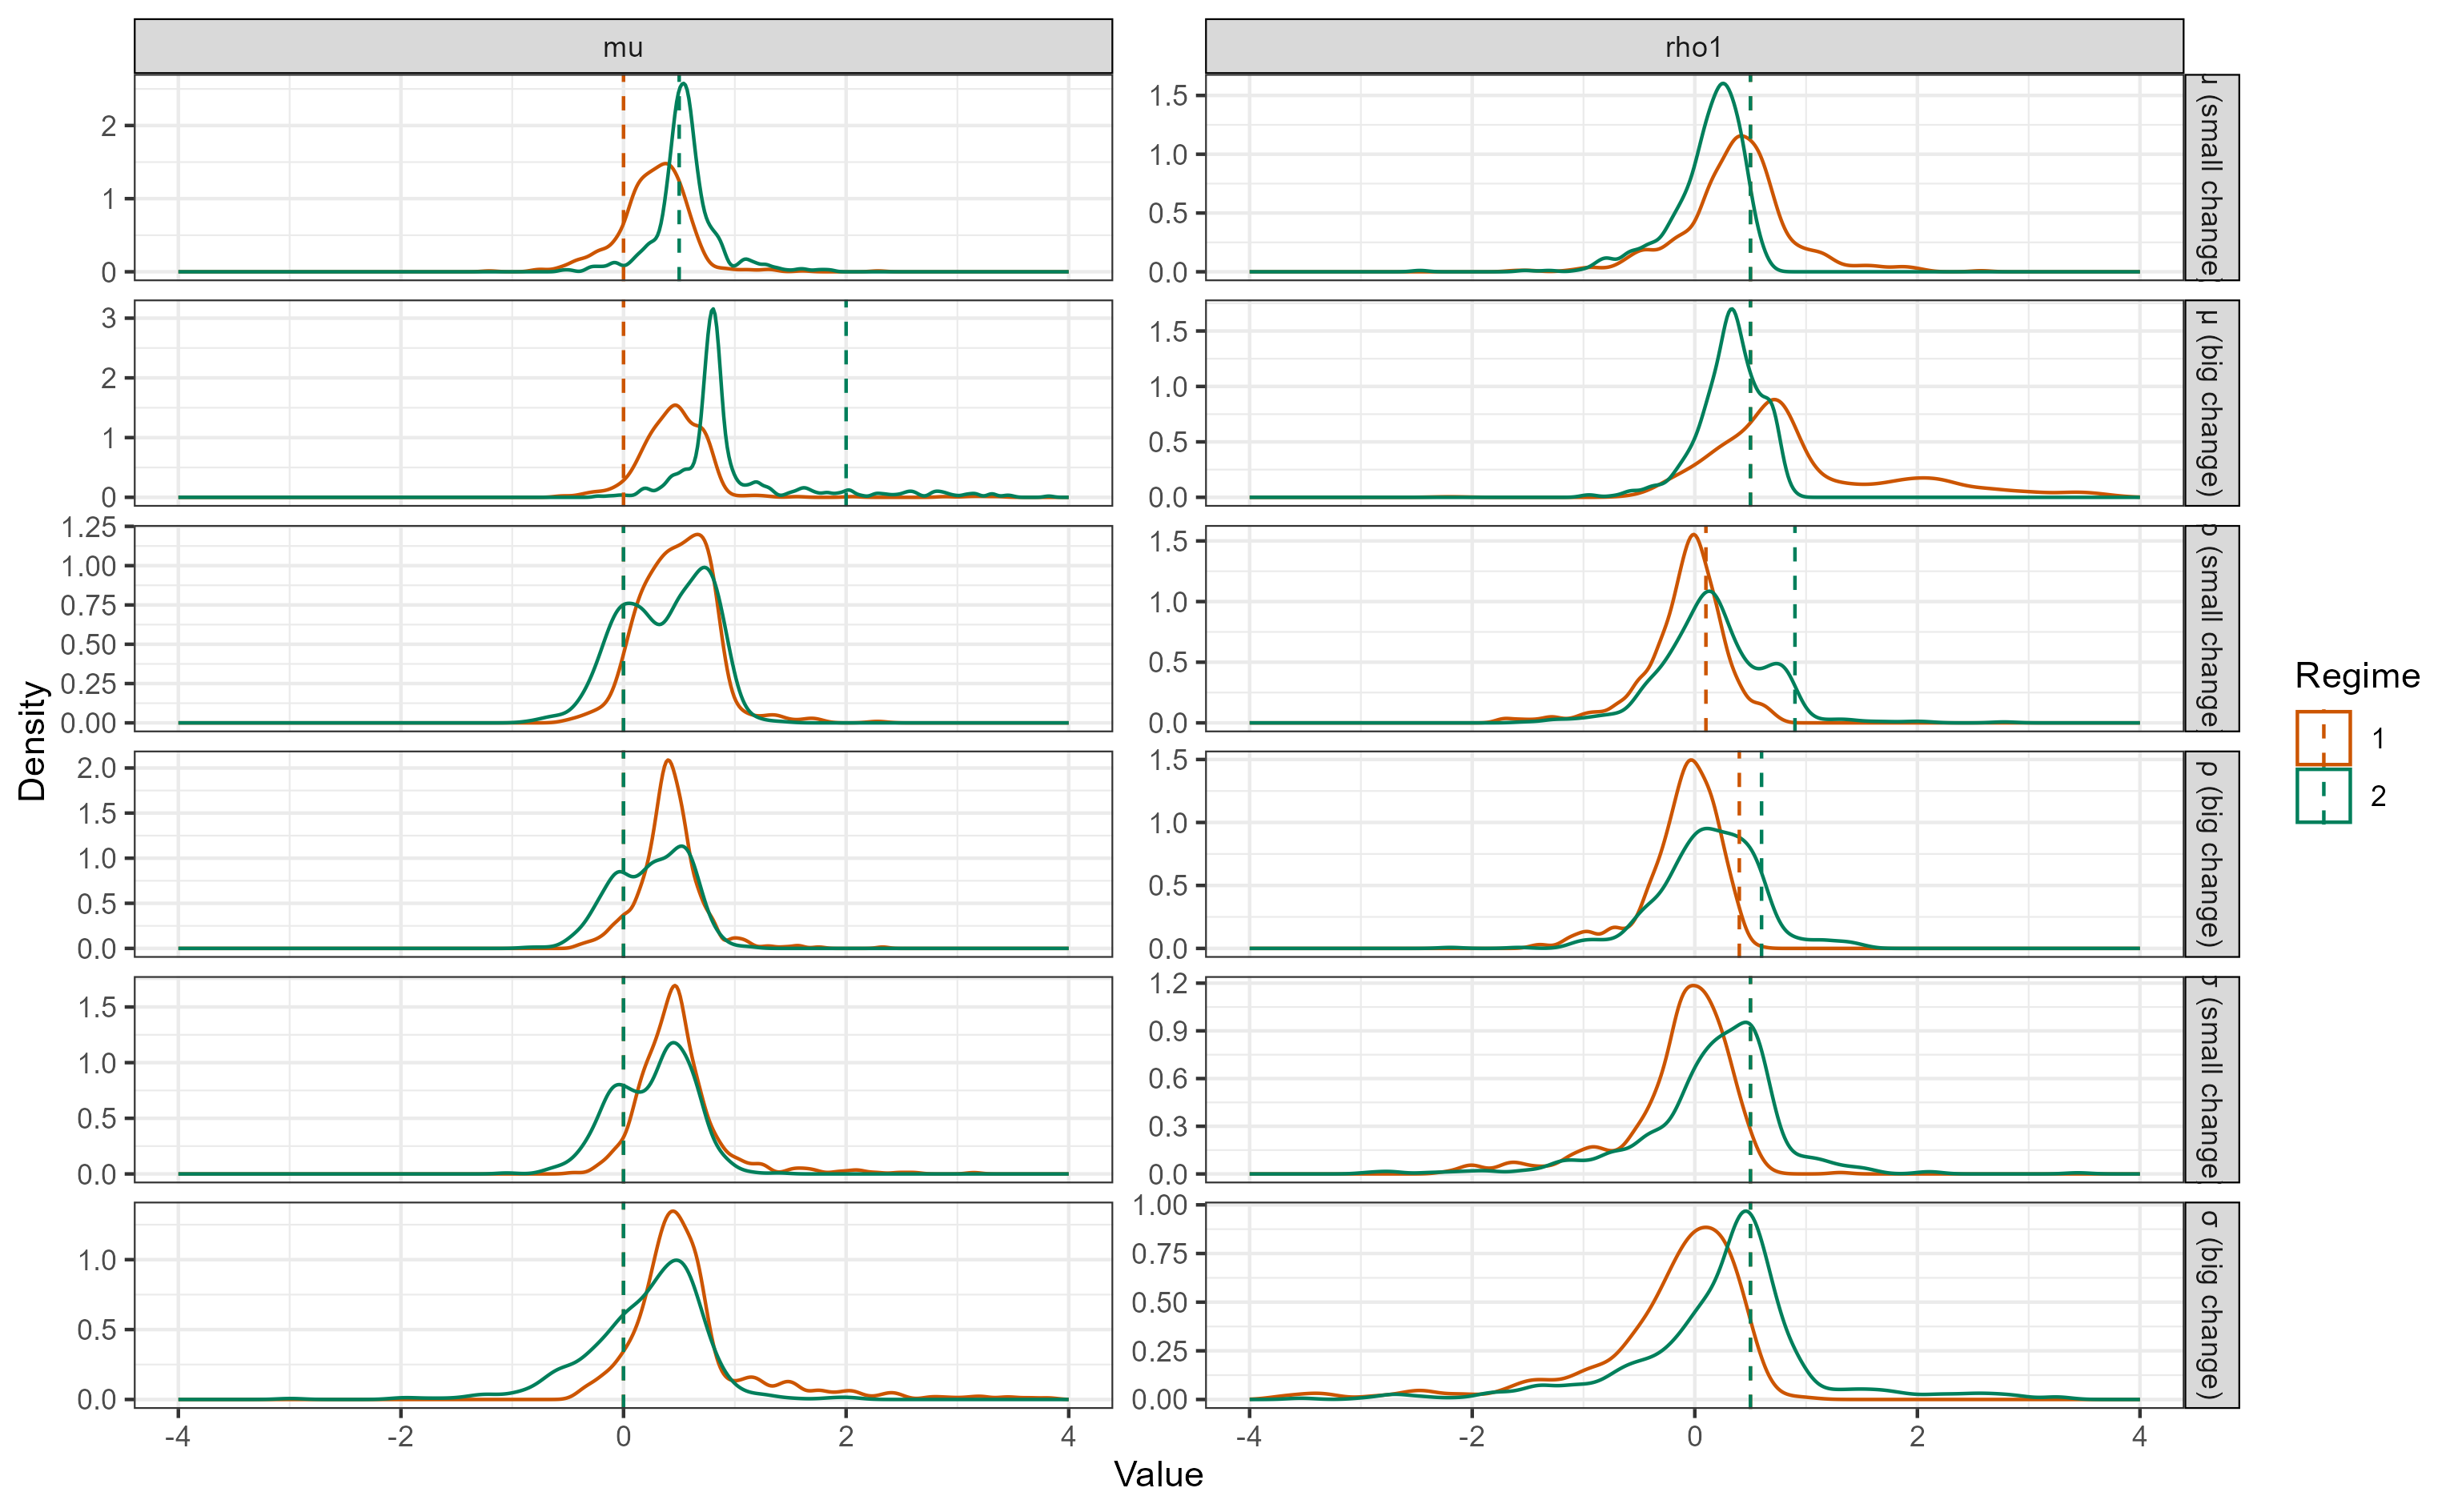
\includegraphics[keepaspectratio]{../../outputs/estimations/coefs-r2_markov_symm_high-r2_sbreak.png}}

}

\end{figure}%
\end{frame}

\begin{frame}{Models - Metrics}
\phantomsection\label{models---metrics}
Now, the same graphs and tables can be created for the estimated values.

At the end, a table comparing the true and estimated metrics shows which
(model, DGP) pairs are unable to capture which characteristics of the
regimes.
\end{frame}

\section{Systematic Analysis}\label{systematic-analysis}

\begin{frame}{Systematic Analysis}
\phantomsection\label{systematic-analysis-1}
Using the stylized facts learned in the exploratory analysis, I do
regression analysis to understand the relationship between performance
and:

\begin{itemize}
\tightlist
\item
  DGP elements.

  \begin{itemize}
  \tightlist
  \item
    Which SGPs, RGPs, and regime natures are more difficult to model?
  \end{itemize}
\item
  Models, and specially their interactions with DGPs.

  \begin{itemize}
  \tightlist
  \item
    Are there models generally more robust to mis-specifications?
  \item
    Which models suffer more from which mis-specifications?
  \item
    What are the role of regime and coefficient identification in this?
  \end{itemize}
\item
  Regime characteristics.

  \begin{itemize}
  \tightlist
  \item
    Do the metrics calculated relate to performance? In which contexts?
  \item
    How does this relate to coefficient and regime \emph{timings}
    identification?
  \end{itemize}
\item
  Other exercises.
\end{itemize}
\end{frame}

\begin{frame}{DGP elements}
\phantomsection\label{dgp-elements}
An important placebo test is to check if the simulation index \(i\) has
no effect:

\begin{equation}
    rmse_{p, i, m} = \beta_0 + \beta_1 i + \varepsilon_{p, i, m}
\end{equation}

The estimated \(\beta_1\) is \(5.0e-5\), with a p-value of \(0.051\).
Given the high power of the test, this seems to be a negligible effect.
\end{frame}

\begin{frame}{Stylized Facts about DGP elements}
\phantomsection\label{stylized-facts-about-dgp-elements}
Consider the categorical variables \(\rgp_{p, i}\) (i.e., vector of
dummies), that indicates which RGP was used, and similar definitions for
\(\sgp_{p, i}\) and \(\mod_{p, i}\).

\begin{equation}
    rmse_{p, i, m} = \beta_0 + \beta_1 \rgp_{p, i} + \beta_2 \sgp_{p, i} + \beta_3 \rgp_{p, i} \cdot \sgp_{p, i} + \varepsilon_{p, i, m}
\end{equation}

Compared to the omitted group of \(\mu\) change and Markov RGP, only the
volatility change has higher RMSE.

All the interactions, except volatility with threshold, have positive
coefficients.
\end{frame}

\begin{frame}{Stylized facts about models}
\phantomsection\label{stylized-facts-about-models}
Then, I analyze the fixed effects of the models. To capture their
sensitivity to mis-specification, we can add interactions between it and
the DGP.

An indicator of correct specification, but this loses information about
the type of mis-specification:

\begin{multline}
    rmse_{p, i, m} = \beta_0 + \beta_1 \rgp_{p, i, m} + \beta_2 \sgp_{p, i} + \beta_3 \rgp_{p, i} \cdot \sgp_{p, i} + \beta_4 \mod_{p, i, m}\\ + \beta_5 \mathbb{1}(\mod_{p, i, m} = \rgp_{p, i}) + \varepsilon_{p, i, m}
\end{multline}
\end{frame}

\begin{frame}{Stylized facts about models}
\phantomsection\label{stylized-facts-about-models-1}
Then, I analyze the fixed effects of the models. To capture their
sensitivity to mis-specification, we can add interactions between it and
the DGP.

Or, a full interaction between model and RGP:

\begin{multline}
    rmse_{p, i, m} = \beta_0 + \beta_1 \rgp_{p, i, m} + \beta_2 \sgp_{p, i} + \beta_3 \rgp_{p, i} \cdot \sgp_{p, i} + \beta_4 \mod_{p, i, m}\\ + \beta_5 \mod_{p, i, m} \cdot \rgp_{p, i} + \varepsilon_{p, i, m}
\end{multline}

One of the most significant results was a particularly bad interaction
between a smooth transition model estimating a structural break RGP.
\end{frame}

\begin{frame}{Coefficients and performance}
\phantomsection\label{coefficients-and-performance}
The regression above can be expanded to include the dispersion of the
estimated coefficients across regimes.

This is a similar exercise as the next one, as the coefficients can also
be seen as regime-conditional metrics themselves.
\end{frame}

\begin{frame}{Regimes characteristics and performance}
\phantomsection\label{regimes-characteristics-and-performance}
To analyze this relation, I propose adding the metrics values as an
additional regressor, and an interaction between it and the model.

As each metric is specific to each SGP, the regressions will be run
separately for each regime nature.

\begin{multline}
    rmse_{p, i, m} = \beta_0 + \beta_1 \rgp_{p, i, m} + \beta_2 \sgp_{p, i} + \beta_3 \rgp_{p, i} \cdot \sgp_{p, i} + \beta_4 \mod_{p, i, m}\\ + \beta_5 \mod_{p, i, m} \cdot \rgp_{p, i} + \beta_6 c_{p, i, m} + \varepsilon_{p, i, m}
\end{multline}

In general, the true vs.~estimated difference of the conditional
metric's dispersion has a positive relation with RMSE.

On the other hand, the absolute dispersions also seem to have a positive
relation with RMSE, which is counter-intuitive.
\end{frame}

\begin{frame}{Other exercises}
\phantomsection\label{other-exercises}
\begin{itemize}
\item
  In the simple setup where ordering regimes is possible, the
  regressions can be run at the \((p, i, m, s)\) level. The results
  would indicate within each regime a model performs better.
\item
  Simiarlly, the metrics can be calculated for the true, estimated
  values, and the difference.
\item
  Results on whether the metrics indeed characterize the regimes, and if
  the models are able to capture that. These could be formalized via
  regressions too.
\end{itemize}
\end{frame}

\begin{frame}{Other exercises}
\phantomsection\label{other-exercises-1}
\begin{itemize}
\item
  The identification performance of the regime variable can be treated
  as a dependent variable, or also as a control.
\item
  Te sensitivity to mis-specification of the number of regimes, can be
  studied via interactions between \(\mathbb{1}(\hat{S} < S)\) and
  metrics' dispersion. if the dispersion across regimes is low,
  mis-specifying the number of regimes should not be as harmful.
\item
  If there is time, test if the practical recommendations help in a
  real-world example, and if the patterns are observed in real data.
\end{itemize}
\end{frame}

\section{Conclusion}\label{conclusion}

\begin{frame}{Summary}
\phantomsection\label{summary}
\begin{itemize}[<+->]
\tightlist
\item
  Regime switching is an interesting way to model non-linearities in
  time series.
\item
  Two focuses: sensibility to mis-specification, and take advantage of
  regime characteristics.
\item
  Framework to generate a diverse menu of DGPs, models, and metrics.

  \begin{itemize}[<+->]
  \tightlist
  \item
    Theoretical framework, simulation methodology, and code
    implementation.
  \item
    Many interesting exercises left aside, but the setup is easily
    expandable.
  \end{itemize}
\item
  Big focus on exploratory analysis.

  \begin{itemize}[<+->]
  \tightlist
  \item
    How DGP behaves, how models interact with them, and how metrics are
    relevant.
  \end{itemize}
\item
  Systematic analysis with potential for practical recommendations.
\end{itemize}
\end{frame}

\begin{frame}
\begin{center}
\Huge Obrigado :)
\end{center}
\end{frame}

\begin{frame}{Referências}
\phantomsection\label{referuxeancias}
\phantomsection\label{refs}
\begin{CSLReferences}{1}{0}
\bibitem[\citeproctext]{ref-BaiPerron1998}
Bai, Jushan, and Pierre Perron. 1998. {``Estimating and Testing Linear
Models with Multiple Structural Changes.''} \emph{Econometrica} 66 (1):
47--78. \url{http://www.jstor.org/stable/2998540}.

\bibitem[\citeproctext]{ref-Chow1960}
Chow, Gregory C. 1960. {``Tests of Equality Between Sets of Coefficients
in Two Linear Regressions.''} \emph{Econometrica} 28 (3): 591--605.
\url{http://www.jstor.org/stable/1910133}.

\bibitem[\citeproctext]{ref-Hamilton1989}
Hamilton, James D. 1989. {``A New Approach to the Economic Analysis of
Nonstationary Time Series and the Business Cycle.''} \emph{Econometrica}
57 (2): 357--84. \url{http://www.jstor.org/stable/1912559}.

\bibitem[\citeproctext]{ref-Medeiros2000}
Medeiros, Marcelo Cunha. 2000. {``Modelos Com Múltiplos Regimes Para
Séries Temporais Limiares, Transições Suaves, e Redes Neurais.''} PhD
thesis, Pontifícia Universidade Católica do Rio de Janeiro, Departamento
de Engenharia Elétrica.
\url{https://research.ebsco.com/c/s7mzkw/search/details/viuhokly5v}.

\bibitem[\citeproctext]{ref-Terasvirta1994}
Teräsvirta, Timo. 1994. {``Specification, Estimation, and Evaluation of
Smooth Transition Autoregressive Models.''} \emph{Journal of the
American Statistical Association} 89 (425): 208--18.
\url{http://www.jstor.org/stable/2291217}.

\bibitem[\citeproctext]{ref-TongLim1980}
Tong, H., and K. S. Lim. 1980. {``Threshold Autoregression, Limit Cycles
and Cyclical Data.''} \emph{Journal of the Royal Statistical Society.
Series B (Methodological)} 42 (3): 245--92.
\url{http://www.jstor.org/stable/2985164}.

\end{CSLReferences}
\end{frame}

\section{Appendix}\label{appendix}

\begin{frame}{Error Diagnostics}
\phantomsection\label{error-diagnostics}
\begin{figure}[H]

\caption{Errors - Correlation across parallelization structure}

{\centering \pandocbounded{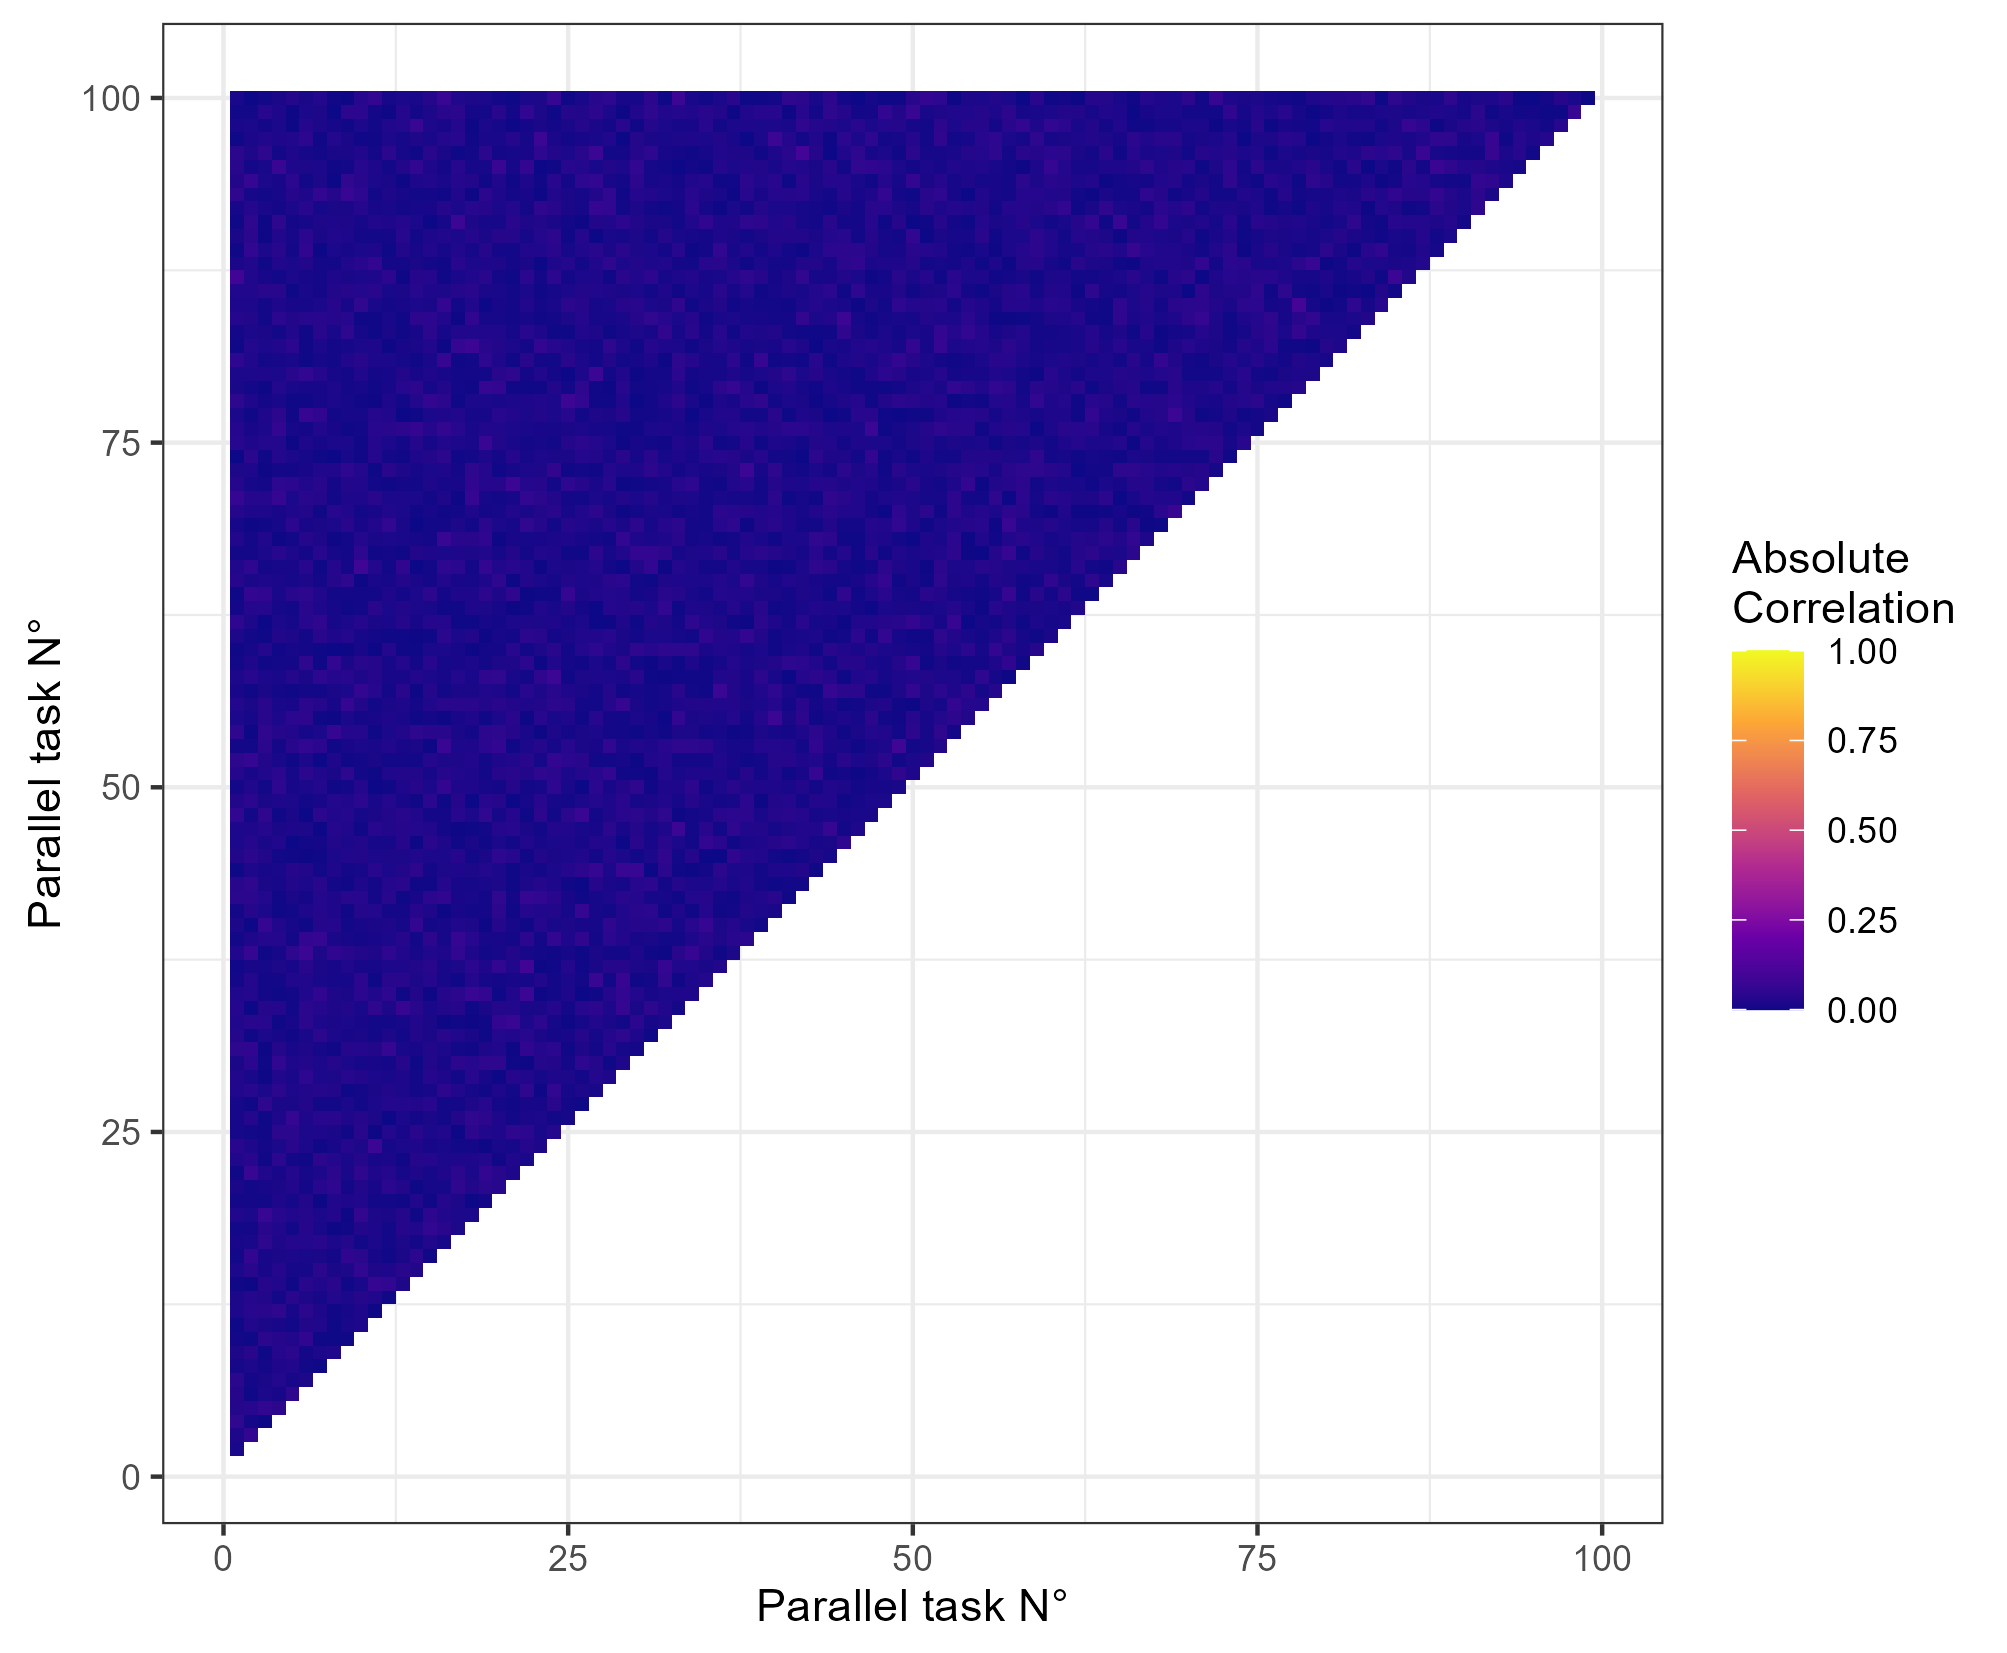
\includegraphics[keepaspectratio]{../../outputs/errors/dependence.png}}

}

\end{figure}%
\end{frame}

\begin{frame}{Error Diagnostics}
\phantomsection\label{error-diagnostics-1}
\begin{figure}[H]

\caption{Errors - Distribution}

{\centering \pandocbounded{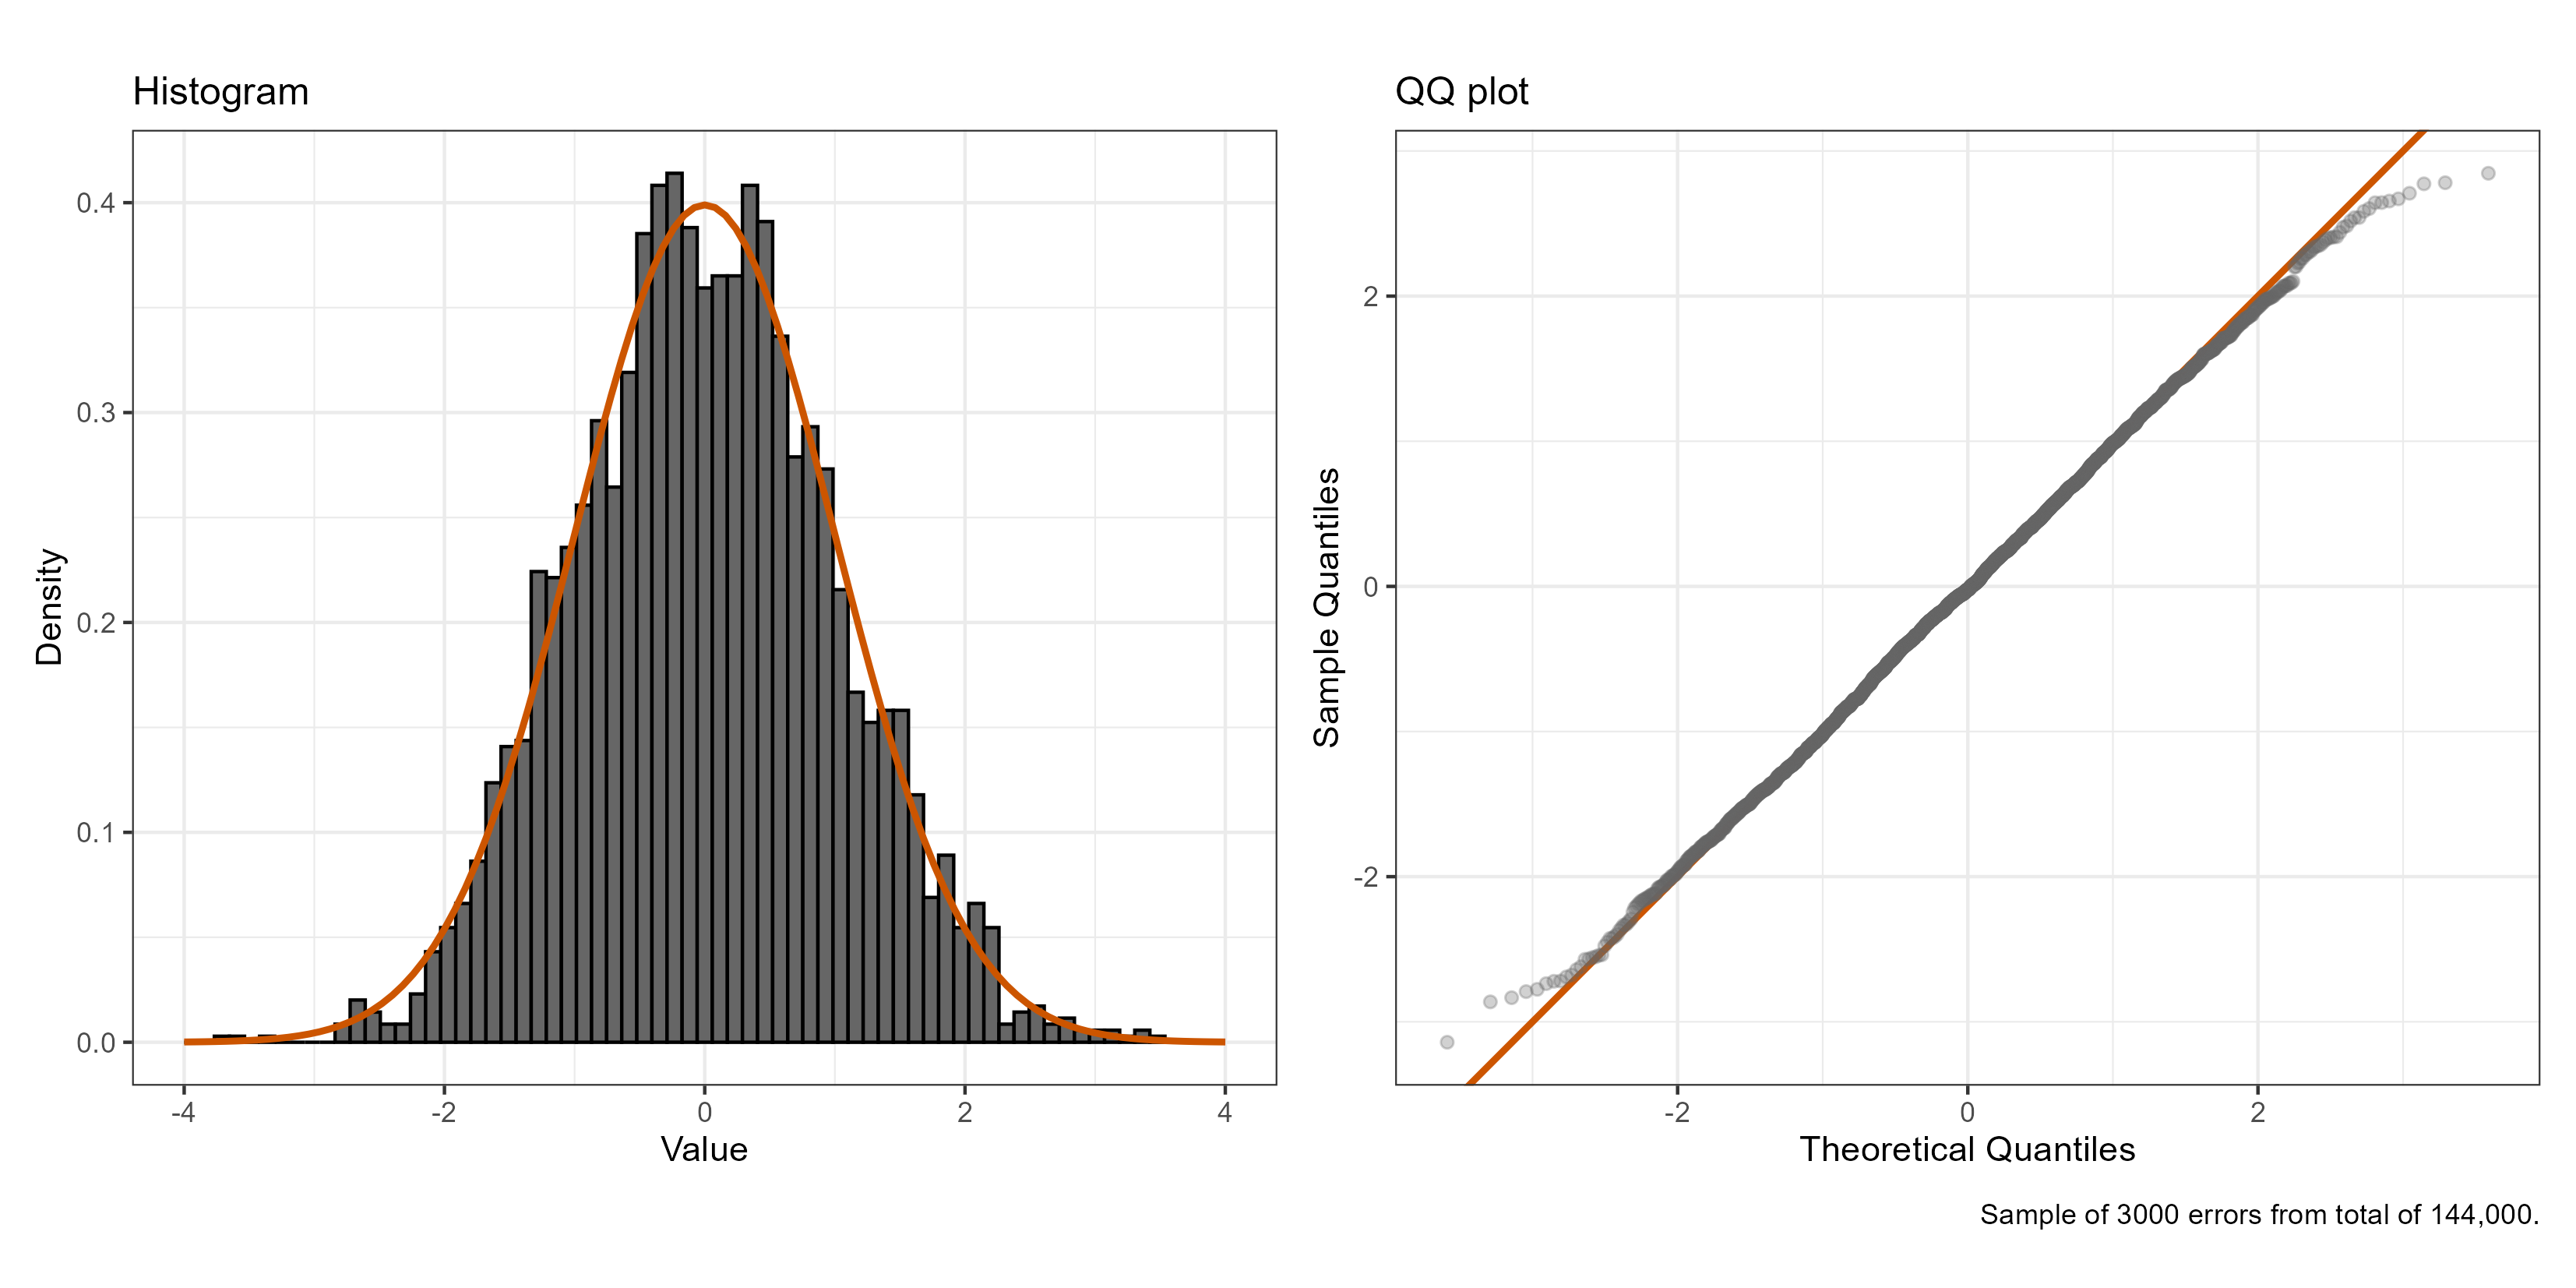
\includegraphics[keepaspectratio]{../../outputs/errors/distribution.png}}

}

\end{figure}%
\end{frame}




\end{document}
